%%%%%%%%%%%%%%%%%%%%%%%%%%%%%%%%%%%%%%%%%
% University/School Laboratory Report
% LaTeX Template
% Version 3.1 (25/3/14)
%
% This template has been downloaded from:
% http://www.LaTeXTemplates.com
%
% Original author:
% Linux and Unix Users Group at Virginia Tech Wiki 
% (https://vtluug.org/wiki/Example_LaTeX_chem_lab_report)
%
% License:
% CC BY-NC-SA 3.0 (http://creativecommons.org/licenses/by-nc-sa/3.0/)
%
%%%%%%%%%%%%%%%%%%%%%%%%%%%%%%%%%%%%%%%%%

%----------------------------------------------------------------------------------------
%	PACKAGES AND DOCUMENT CONFIGURATIONS
%----------------------------------------------------------------------------------------

\documentclass[12pt,a4paper]{article}

%\usepackage[version=3]{mhchem} % Package for chemical equation typesetting
%\usepackage{siunitx} % Provides the \SI{}{} and \si{} command for typesetting SI units
\usepackage{graphicx} % Required for the inclusion of images
\usepackage{geometry}
%\usepackage{natbib} % Required to change bibliography style to APA
%\usepackage{amsmath} % Required for some math elements 
%\usepackage{enumerate}
\usepackage{indentfirst}
\usepackage{listings}
\providecommand{\keywords}[1]{\textbf{\textit{Keywords:}} #1}
\lstset{
  basicstyle=\ttfamily,
  columns=fullflexible,
  frame=single,
  breaklines=true,
%  postbreak=\mbox{\textcolor{red}{$\hookrightarrow$}\space},
}
%\usepackage{biblatex}
%\addbibresource{report.bib}
%\setlength\parindent{24pt}


%\renewcommand{\labelenumi}{\alph{enumi}.} % Make numbering in the enumerate environment by letter rather than number (e.g. section 6)

%\usepackage{times} % Uncomment to use the Times New Roman font

%----------------------------------------------------------------------------------------
%	DOCUMENT INFORMATION
%----------------------------------------------------------------------------------------

\title{Improvements for Congestion Control Algorithms in Large-Scale Data Center Network \\ Algorithm Adjustment for DCQCN \\ undergraduate dissertation} % Title

\author{Yuchen \textsc{Yang}} % Author name

\date{\today} % Date for the report

\begin{document}

\maketitle % Insert the title, author and date

\begin{center}
\begin{tabular}{l}
141242048 \\
Kuang Yaming Honors School, Nanjing University \\
ranchyang96@gmail.com \\
Instructor: Professor Chen Tian
\end{tabular}
\end{center}


\begin{abstract}
	Modern data centers are experiencing a fierce increase in scale and traffic bandwidth.
	Remote Direct Memory Access (RDMA) permits high-throughput, low-latency networking,
	which is especially useful in such a large-scale scenario.
	The most primitive method (like TCP/IP stack) for congestion control is to drop packets when the receiver buffer is full.
	Later we have Priority-based Flow Control (PFC) to generate congestion information in ACKs.
	Before this paper, we have Data Center Quantized Congestion Notification (DCQCN) which uses the state-of-the-art scheme for congestion control.
	However, we may find DCQCN incapable of some large-scale traffic scenarios.
	In this paper, we analyze the drawbacks of DCQCN.
	At the same time, we present our improvements to DCQCN and name it DCQCN+.
	Improvements mainly focus on the adaptive increasing step and intervals.
	We have implemented them on testbeds and NS3 simulation.
	Our method has 10 times smaller latency than DCQCN under large-scale conditions (incast of over 400:1) and 4 times larger flow capability than DCQCN.
	While in small incast cases, we have similar performance with DCQCN.
	This paper additionally focuses on my own work, about the testbed implementation and configurations of the method.
	It actually includes many detailed methods used for execution of experiments and detailed information about testbed experiment results.
\end{abstract}

\keywords{Data Center Network; Congestion Control; DCQCN}

\tableofcontents
\listoffigures
\listoftables

\newpage
\section{Introduction}

Modern data centers are experiencing a fierce increase in both scale and bandwidth.
To be more specific, we find following features of data centers nowadays:
\begin{enumerate}
	\item Small latency: $<100\mu s$
	\item High bandwidth: $10/40~100Gbps$
	\item Shallow buffer: $<300MB$ for ToR
	\item Large scale: $>10000$ machines
\end{enumerate}

As we know, data centers need small RTTs (some even tens of microseconds),
so abilities to handle burst flows for incasts and support the equality and balancing for concurrent flows matter a lot.
Traditional TCP/IP stack surely can't do the job.
When encountering a large number of concurrent flows, TCP may choose to drop packets when the receiver buffer is full.
That's not tolerable for sure in data centers since data centers require the lossless network to ensure the security and accuracy of large-scale traffic.
Then the first idea coming is to find a way to predict the congestion of the receiver end.
We hope to let the sender get some information about the receiver.

Then we get Explicit Congestion Notification (ECN) \cite{ECN} at the beginning.
This method uses a mark in the IP header of the ACK.
If the receiver dropped a packet, it echoes the congestion indication to the sender, so that the sender can reduce its sending rate.
Such ECN flags indicate the existence of congestion from receiver side after congestions have already happened.
ECN somehow relieves the congestion and makes the receiver side drop fewer packets, but this still can't be lossless.

Later Quantized Congestion Notification (QCN) \cite{QCN} is developed.
QCN enables the switch to control the packet sending rate of an Ethernet source whose packets are traversing the switch.
This maintains a stable queue occupancy and is easy to be implemented on hardware.
QCN is also applicable for multiple flows in the same port.

Priority-based Flow Control (PFC) \cite{PFC} applies the PAUSE frame to make things better.
PAUSE is used by the receiver to send feedback to the sender about the remaining buffer space.
PFC actually divide services into 8 classes to make the feedback information more accurate.
Since the PAUSE frame carries more information, senders can know the exact remaining space in receiver buffer.
Thus the reaction on sending rate can be more accurate.
However, this method can't be specific on flows but only on ports, which is usually combined with ECN to make it work better.

Data Center TCP (DCTCP) \cite{dctcp} begins to react in proportion to the extent of congestion instead of presence.
This congestion level is conveyed by ECN marks carried by packets.
These ECN marks are based on instantaneous queue length.

Before this paper, we have Data Center QCN (DCQCN) \cite{dcqcn} which handles congestion better and is the basic point of our work.
DCQCN is the application of QCN on data centers, which divides the overall algorithms into three parts.
It's kind of combination of Data Center TCP (DCTCP) and PFC.
A brand-new concept mentioned here is Congestion Notification Packet (CNP), which functions similarly as PAUSE frame in PFC but carries more informations.
CNP packets are actually sent by NP which is the receiver end.
Each time when a packet with ECN mark is got and there are no CNP packets sent during the last interval period, a CNP is sent to notify the
sender.
Here the interval period mentioned is usually an interval set up in advance by hardware to make sure that there won't be a CNP burst on
RP side.
This interval is also greatly limited by hardware ability.
Detailed information is also be mentioned in later sections.

However, DCQCN has performance problems when large-scale incasts happen.
When many hosts send data simultaneously to a same receiver, incasts happen \cite{ICTCP}.
Such traffic pattern is commmon for many data center applications such as MapReduce shuffling \cite{MapReduce}
and distributed Storage such as Ceph \cite{Ceph}.
This leads to large queue length of the receiver buffer, which will greatly increase queueing latency.
Also, this can generate PFC bursts according to \cite{Guo2016RDMA}, which may generate victim flows.


In the end here is a brief introduction of the most important points about our new method DCQCN+.
DCQCN+ deploys dynamic rate control mechanisms to adapt to incast of different scales instead of the fixed rate control for DCQCN.
What I'm in charge of are the testbed configuration and experiments.

The paper is organized as follows.
In Section 2 we introduce the background of the project.
In Section 3 we present limitations of DCQCN and necessity for improvements.
In Section 4 we show possible improvements for DCQCN.
In Section 5 I display detailed methods used for testbed experiments.
In Section 6 we show the results of experiments.
In Section 7 there are some discussions and future work.

\newpage
\section{Background}
\subsection{Mellanox switch and ConnectX-4}
In the testbed experiments, we are using Mellanox SN2700 switch and ConnectX-4 Network Interface Cards.
Mellanox SN2700 carries a huge throughput of 6.4Tb/s, 32 ports at 100GbE.
The port speed can actually vary from 10Gb/s, 25Gb/s, 40Gb/s and 100Gb/s.
All 32 ports are connected to 16 machines inside our testbed with 2 each, but only 9 ports on 9 separate machines are used inside our
testbed experiments.

ConnectX-4 EN adapter can support 100Gbps Ethernet Connectivity.
Its Virtual Protocol Interconnect also supports EDR 100Gbps InfiniBand traffic.
We have ConnectX-4 adapters on all machines in our testbed.
Additionally, we have tested the ability of ConnectX-5 adapters on a new testbed about the Congestion Notification Packet generation
ability.
This is described in later sections.

\subsection{InfiniBand}

InfiniBand is a computer-networking communication standard used in high-performance computing.
Such standard supports features of high throughput and low latency.

It can actually work both among and within computers. It's most commonly used in supercomputers and data centers.

In later testbed experiments, commands ''ib\_send'' includes IB which is the abbreviation for InfiniBand.

\subsection{Remote Direct Memory Access}
Remote Direct Memory Access almost satisfies all the demands for data center networks.
It permits high throughput and low latency.
Similar to Direct Memory Access, RDMA actually allows user-space applications to directly read or write without the operation from
any operating systems.
Such network feature omits the possible copies inside systems, thus performs better inside data centers.

\subsection{RoCE v2}

The complete name is RDMA over Converged Ethernet version 2 \cite{RoCEv2}.
RoCE is a network protocol that allows RDMA over an Ethernet network
which has advantages of low latency, low CPU usage and high bandwidth.

RoCE v1 is an Ehternet link layer protocol which allows traffic under the same Ethernet domain.
RoCE v2 is an Internet layer protocol which permits routing.
We are using RoCE v2 to make improvements in Internet layer.

\subsection{Priority-based Flow Control}
Priority-based Flow Control ensures the lossless feature for RDMA.
No buffer packet overflow is a must for data center networks.

However, PFC actually does nothing to make the latency low.
When the receiver buffer is almost full, the packets inside the buffer queue up for a long time which makes the queueing latency
extremely high.
Such unfairness, victim flows \cite{dcqcn}, deadlock \cite{Guo2016RDMA} and high latency are fatal to data centers and we hope to make up the drawbacks.

\subsection{Explicit Congestion Notification}
Explicit Congestion Notification is designed to indicate congestion to the sender.
An ECN-aware router may set a mark in the IP header instead of dropping a packet in order to signal impending congestion.
The receiver of the packet echoes the congestion indication to the sender,
which reduces its transmission rate if it detects a dropped packet.

\subsection{Data Center TCP}

DCTCP has 2 brand-new features. It somehow reveals the basic points of DCQCN.

The first is reacting in proportion to the extent of congestion but not its presence.
It's actually reducing window size based on the fraction of marked packets.

The second is that ECN marks are based on instantaneous queue length.
It provides fast feedback to better deal with bursts and also simplifies the hardware implementation.

\subsection{DCQCN}
Data Center Quantized Congestion Notification is explained in detail by \cite{dcqcn}.
Here I generally describe the mechanisms used in DCQCN.

Three parts of algorithms are developed.
The parts are Congestion Point (CP), Reaction Point (RP) and Notification Point (NP),
which are switches, senders and receivers respectively.
Both the switch and end points participate in to make things right.

For NP, i.e. receivers, they need to generate and send CNP when a packet with ECN mark and there is no CNP sent during the last interval.
CNPs are generated by receivers, indicating the remaining size of the receiving buffer.

For CP, a function of ECN marking probability P is related with Egress Queueing size S:

for $0<S<K_{min}$, $P = 0$

for $K_{min}<S<K_{max}$, $P = (S - K_{min})/(K_{max} - K_{min})*P_{max}$

for $S>K_{max}$, $P = 1$

which is shown in Figure ~\ref{fig:ECNMarking}.

\begin{figure}[h!]
	\begin{center}
		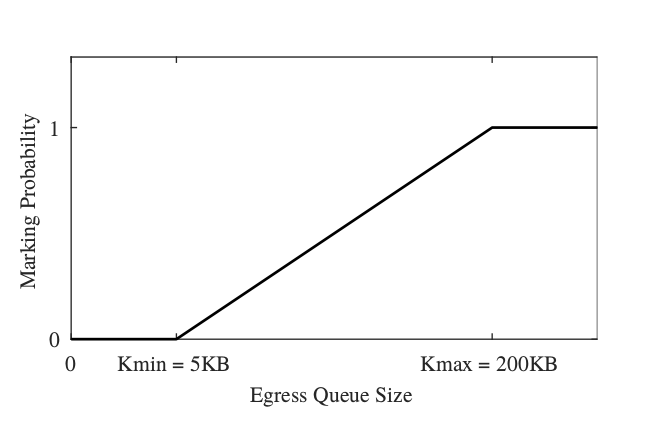
\includegraphics[width=5in]{ECNMarking}
		\caption{ECN Marking Probability for CP in DCQCN}
		\label{fig:ECNMarking}
	\end{center}
\end{figure}

Such marking probability is a brandnew idea from QCN.
Previously marking ECN or not is a fixed thing without possibility.
Such 0/1 resolution for ECN is not proper because that may cause the late reaction from senders.

\subsection{Other related work}

All the congestion control schemes we mention here start to react the congestion after it happens.
TIMELY\cite{TIMELY} is another congestion control scheme for RoCEv2 that is based on RTT reaction.
\cite{DCQCNandTIMELY} compares DCQCN and TIMELY on different aspects of performance,
and claims that ECN is a better congestion signal compared to delay.
\cite{AnalysisofDCTCP},\cite{AnalysisofQCN} and \cite{DCQCNandTIMELY} analyze the stability and convergence of similar congestion control schemes.
\cite{ECNMarking} improves ECN with Micro-burst traffic using Combined Enqueue and Dequeue Marking (CEDM).
\cite{AnalysisofECN}\cite{AnalysisofSmallBuffers} give theoretical analysis of ECN.

\subsection{Python Paramiko Library}

The most used library in my scripts is Python Paramiko
which provides the secure connection for remote command execution and file transmission.
It's actually a Python implementation of SSHv2 protocol, providing functions of both server and client.
To be more specific, I contracted them to three functions,
one for remote command execution and the other two for file transmission between local and remote machines.
Every remote command execution here is using SSH protocol and thus my functions can be implemented by Python Paramiko.

\subsubsection{Remote Command Execution}
The first one is the code listed here, used for remote command execution.

\begin{lstlisting}[language=Python]
def ssh1(ip,username,passwd,cmd):
    try:
        ssh=paramiko.SSHClient()
        ssh.set_missing_host_key_policy(paramiko.AutoAddPolicy())
        ssh.connect(ip,22,username,passwd,timeout=5)
        for m in cmd:
            print(ip,m)
            stdin,stdout,stderr=ssh.exec_command(m)
            err=stderr.readlines()
            for e in err:
                print(ip,e)
        ssh.close()
    except:
        print(ip,'ssh1 Error')
\end{lstlisting}

The commands are actually stored inside the array of ''cmd''.
All commands inside ''cmd'' are executed in sequence.
The results are returned from stdin, stdout and stderr.

Apart from the basic points, another tough point is fetching responses of command executions.
We need to record standard output and sometimes error of the command execution.
In Python Paramiko, it's packed as the return value of ''exec\_command''.
We fetch the responses from ''readlines'', both error messages and output messages can be collected.

\subsubsection{Fetch file from remote end}
The scripts run on the middle machine, which needs to fetch files like Pcap from testbed machines.

\begin{lstlisting}[language=Python]
def ssh2(ip,port,username,passwd,remote_file,local_file):
    try:
        transport=paramiko.Transport((ip,port))
        transport.connect(username=username,password=passwd)
        sftp=paramiko.SFTPClient.from_transport(transport)
        sftp.get(remote_file,local_file)
        sftp.close()
        transport.close()
    except:
        print(ip,'ssh2 Error')
\end{lstlisting}

After building a SFTP connection, we can easily fetch the necessary files.

There is another problem about the file location.
Sadly after using the scripts, relative file locations don't work at all.
The execution position is not the same with the scripts' location.
We need to set up the absolute locations for both files so that the scripts can be run successfully.

\subsubsection{Send file to remote end}
The scripts send specific files to remote ends.
In my experiment, it's used to send Pcap files from the middle machine to my local machine for packet processing.

\begin{lstlisting}[language=Python]
def ssh3(ip,port,username,passwd,local_file,remote_file):
    try:
        transport=paramiko.Transport((ip,port))
        transport.connect(username=username,password=passwd)
        sftp=paramiko.SFTPClient.from_transport(transport)
        sftp.put(local_file,remote_file)
        sftp.close()
        transport.close()
    except:
        print(ip,'ssh3 Error')
\end{lstlisting}

\subsubsection{Filtering of outputs}
When printing these responses on screen, we filter the necessary messages out.
Sometimes we need several trials to find out the most useful information.
With the useful lines always having similar starting words, we can redirect them to files for later checks.

\subsection{Python Multithreading}

This point is more common for other programming cases.

In the original version, the time for running is previously estimated.
Thus the execution time of the program is greatly increased or a command is run before its previous steps are finished.
Function ''join'' can correctly sequence all the steps in the program.

In my scripts, there are 5 stages divided and each is ensured to be completed with a series of ''join''.
Thus we don't need to estimate the wait time and can safely wait and watch possible error messages printed on the screen.

The following shows a detailed part about how the scripts are working.

\begin{lstlisting}[language=Python]
    for i in mac[:j]:
        ip='192.168.1.'+str(i)
        b[i]=threading.Thread(target=ssh1,args=(ip,username,passwd,cmd0))
        b[i].start()

    for i in mac[:j]:
        b[i].join()
\end{lstlisting}

The list ''mac'' stores all the last part of the IP of remote machines.
To run commands simultaneously on all remote machines, we use this part of the code.
Thus the execution can be ensured to start at almost the same time and the next steps 
will be executed after all these commands are completely executed.

\subsection{Gnuplot}

In my experiments, most figures are drawn using Gnuplot \cite{Gnuplot}.
Gnuplot is a a portable command-line driven graphing utility for Linux and many other platforms.
All the experiments are done under Linux and it's easier to install and use since it's command-line functions are easy for me.
Also, Scripts can also be applied so that large amount of figures can be drawn without the need
to rewrite many possible plotting scripts.

\subsection{Awk}

Awk \cite{Awk} is a programming language designed for text processing and typically used as a data extraction and reporting tool for Unix-like systems.
With similar reason for Gnuplot, I choose Awk to make things easier.

\newpage
\section{Problems of DCQCN}

The major problem for DCQCN is the failure of dealing with large-scale incast traffic.
Both in simulation \cite{NS3} and testbed experiments show that the switch buffer queue length remains high
after a large burst at the beginning.

\subsection{Testbed experiments}

We use the topology from Figure ~\ref{fig:Topology}.
Actually, there are 9 hosts and one of them is the receiver, the rest of them are senders.
For large-scale congestion, we use Tcpdump \cite{Tcpdump} to capture packets for throughput statistics.
We also turn on sniffer on NICs to make sure that traps are triggered in Lipcap.

In testbed experiments, we actually find that when the flow number is under 400, the queue length will go down after 2 or 3 seconds.
Here the flows are continuous InfiniBand traffic lasting for about 80 seconds and they are started at approximately the same time.
There could be some difference in starting times but within 1 second.
This means that when the flow number is not large, convergence should be reached within 2 seconds.

However, when we start over 400 flows, the high queue length lasts until the end of all flows.
Convergence fails to be reached when the flow number gets really large.

Nowadays the tendency is that scale of data centers grow larger and larger which gives much pressure on data center networks.
Such a long queue length surely lead to high network latency and unfairness.
Thus the demand for data center network is not met.

\subsection{NS3 Simulation}

Here we use the DCQCN simulation \cite{DCQCNsim} released by Yibo Zhu, the designer of DCQCN.

In simulation results, we find even worse convergence effect.
We can see that DCQCN fails to converge under 10Gbps links in Figure ~\ref{fig:DCQCNfail1}
and under 40Gbps links in Figure ~\ref{fig:DCQCNfail2}.
The failure of 10Gbps starts from 80 flows and that of 40Gbps from 160 flows.
All the parameters used here are default parameters on Mellanox official forum \cite{MellanoxOfficial}.

\begin{figure}[h!]
	\begin{center}
		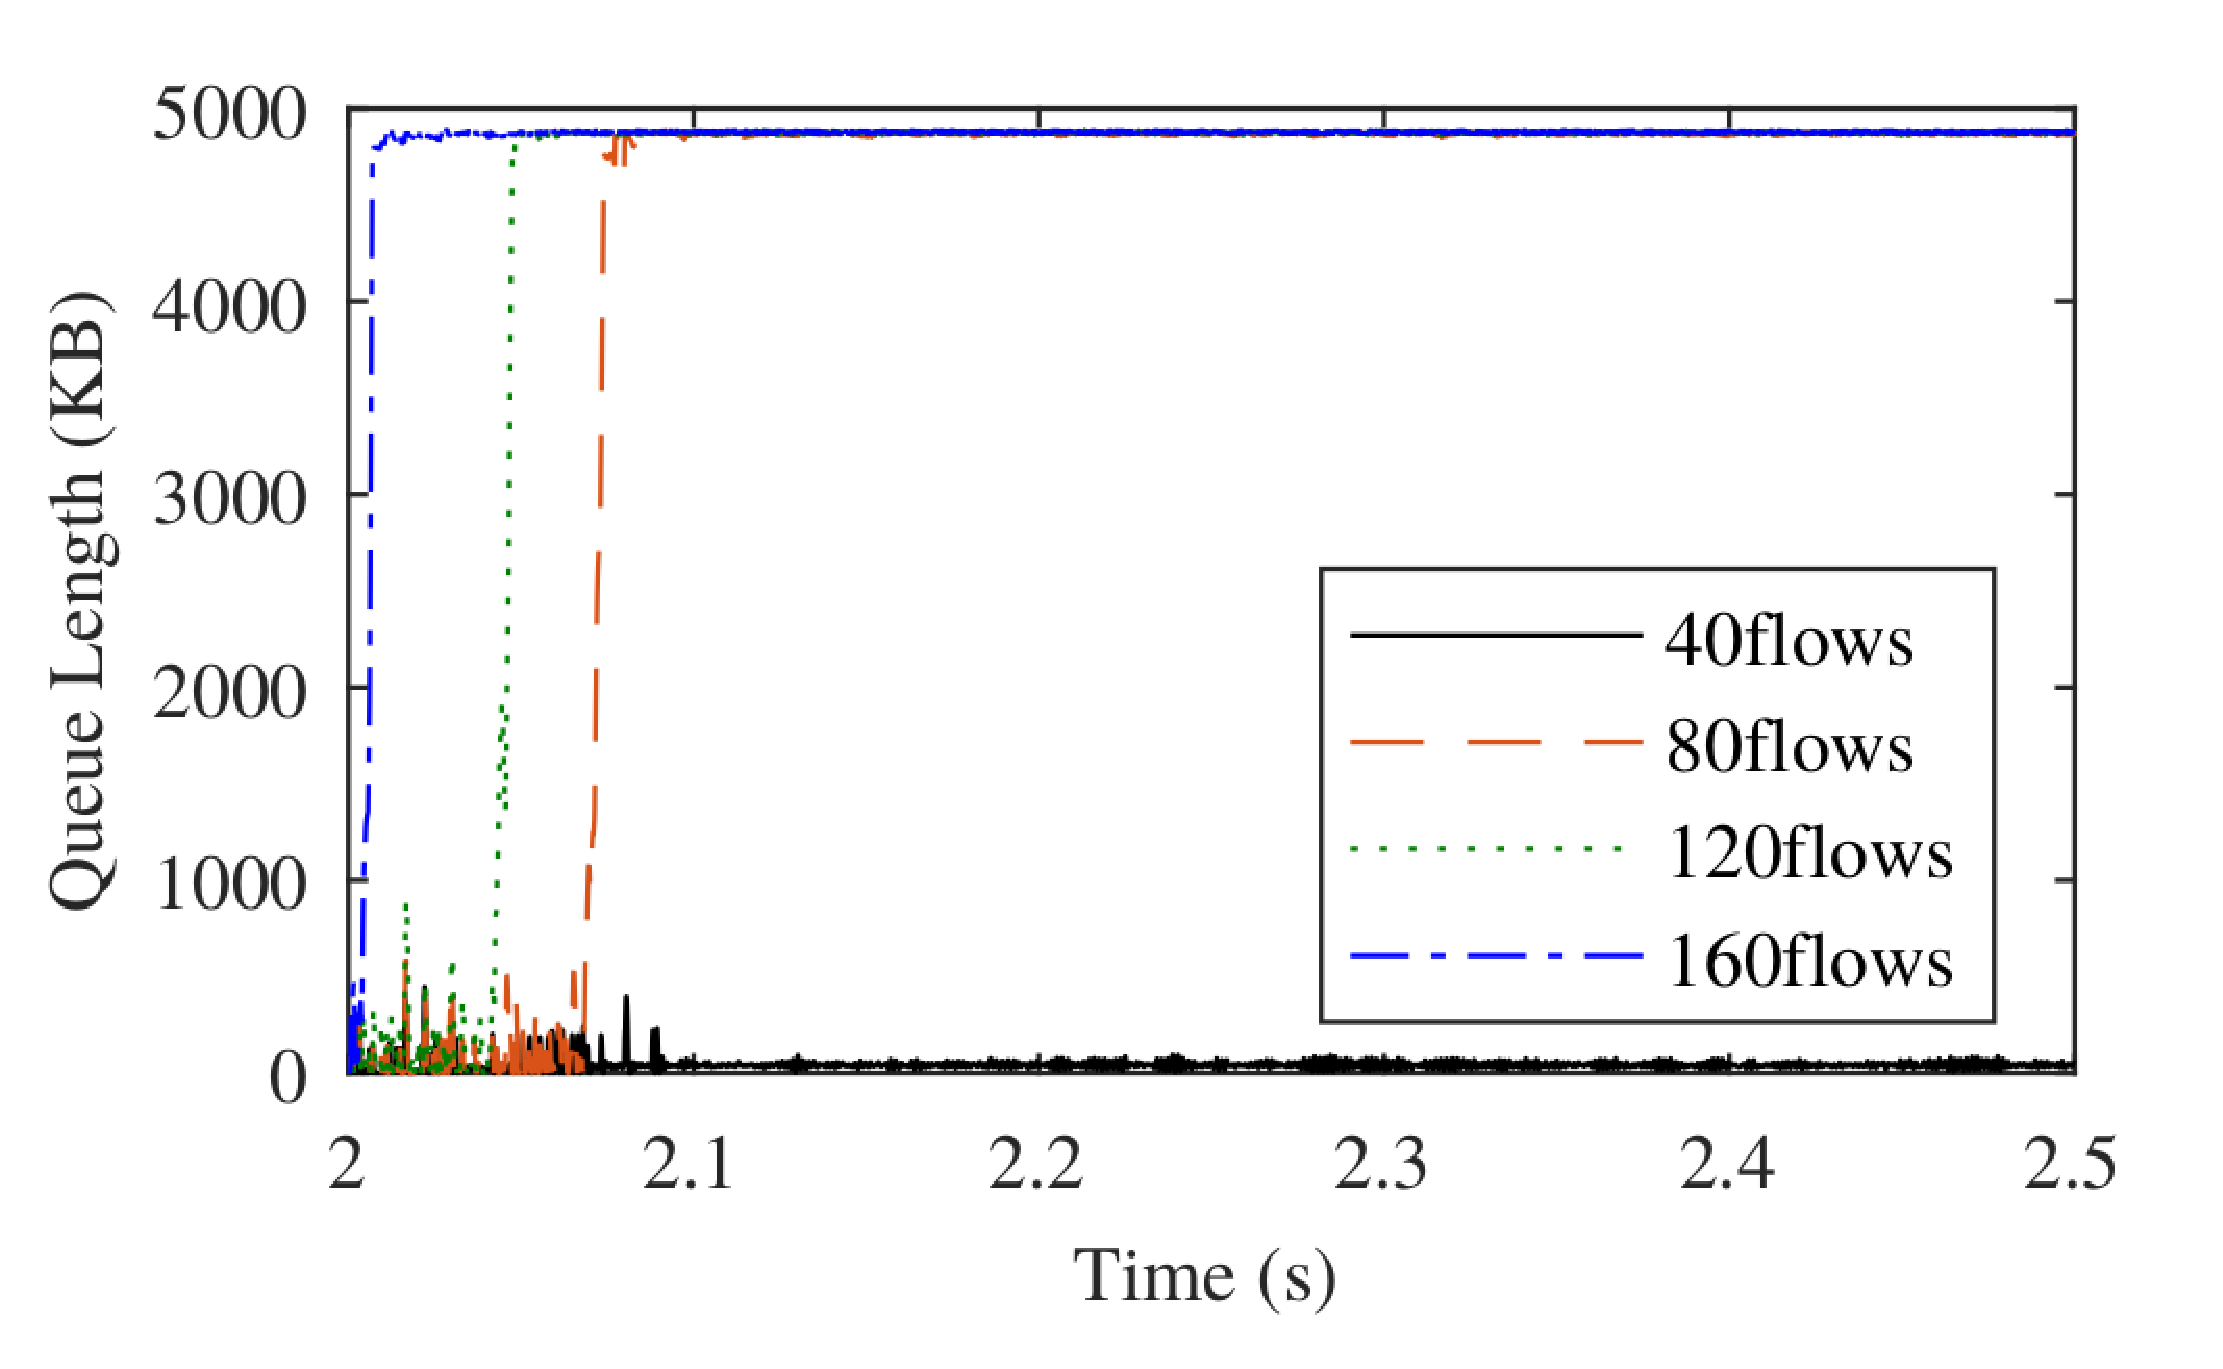
\includegraphics[width=5in]{DCQCNfail1}
		\caption{DCQCN fails to converge in 10Gbps links}
		\label{fig:DCQCNfail1}
	\end{center}
\end{figure}

\begin{figure}[h!]
	\begin{center}
		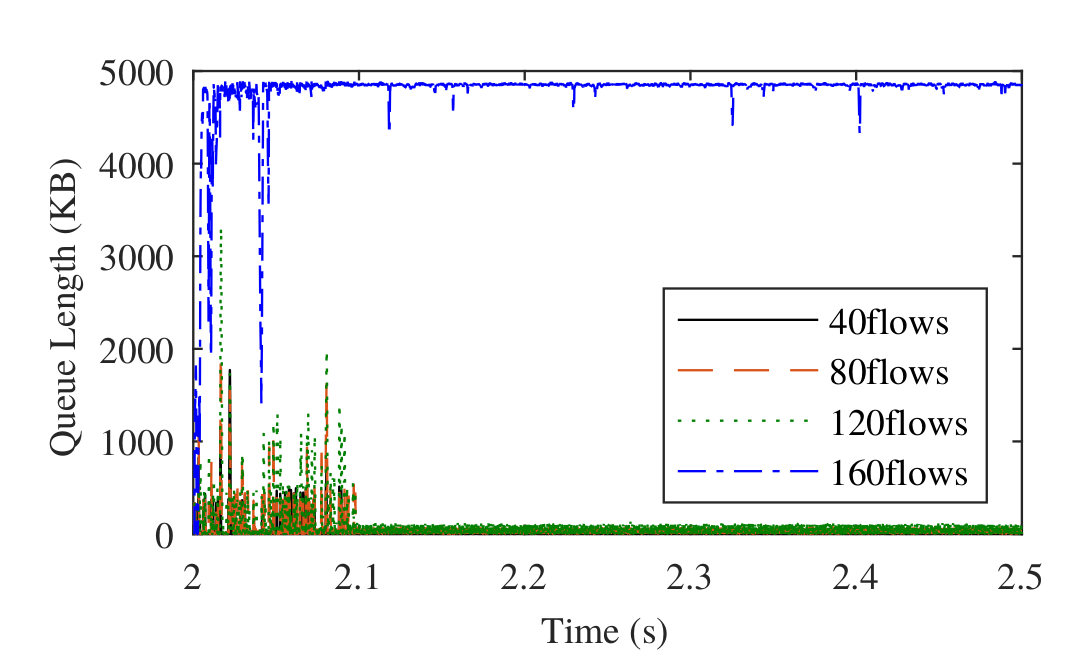
\includegraphics[width=5in]{DCQCNfail2}
		\caption{DCQCN fails to converge in 40Gbps links}
		\label{fig:DCQCNfail2}
	\end{center}
\end{figure}

\subsection{Difference between DCQCN and ConnectX-4 implementation}

When tested in testbeds, we find something really strange.

When we set all the links to 10Gbps in a topology shown in Figure ~\ref{fig:Topology},
we can see that at the beginning the sending rate increases at line rate.
However when we change the link speed to 40Gbps or 100Gbps with the same topology,
we see the speed increasing tendency similar to the 10Gbps one, which is not at line rate.

There must be some implementation difference between the ConnectX-4 and the original DCQCN.
I guess the possible reason for that is, at the creation time of DCQCN, 10Gbps is a suitable upper bound of line rate start.
10Gbps is also a maximal flow rate under DCQCN's control, thus the speed gaining scheme can be suitable for a long time.

If we take a look at the parameter differences, we find the contrast in Table ~\ref{tab:contrast}.
\begin{table}[h!]
	\begin{center}
		\caption{Parameter differences between DCQCN and ConnectX-4}
		\label{tab:contrast}
		\begin{tabular}{|c|c|c|c|}
			\hline
			ConnectX-4 parameter & ConnectX-4 value & DCQCN parameter & DCQCN value\\
			\hline
			rpg\_timer\_reset & $300\mu s$ & Timer & $55 \mu s$\\
			\hline
			rpg\_byte\_reset & 2MB & ByteCounter & 10MB\\
			\hline
			rpg\_ai\_rate & 5Mbps & Additibe Increase Step & 40Mbps\\
			\hline
			rpg\_hai\_rate & 40Mbps & Hyper Increase Step & 100Mbps\\
			\hline
			min\_time\_between\_cnps & $0\mu s$ & CNP interval & $50\mu s$\\
			\hline
			rate\_reduce\_monitor\_period & $4\mu s$ & - & - \\
			\hline
		\end{tabular}
	\end{center}
\end{table}

These paremeters vary a lot so the internal implementation of ConnectX-4 and Mellanox is a mystery.

The difference becomes more apparent from throughput differences.
Figure ~\ref{fig:cx4imp} shows the DCQCN implementation on ConnectX-4 adapters.
\begin{figure}[h!]
	\begin{center}
		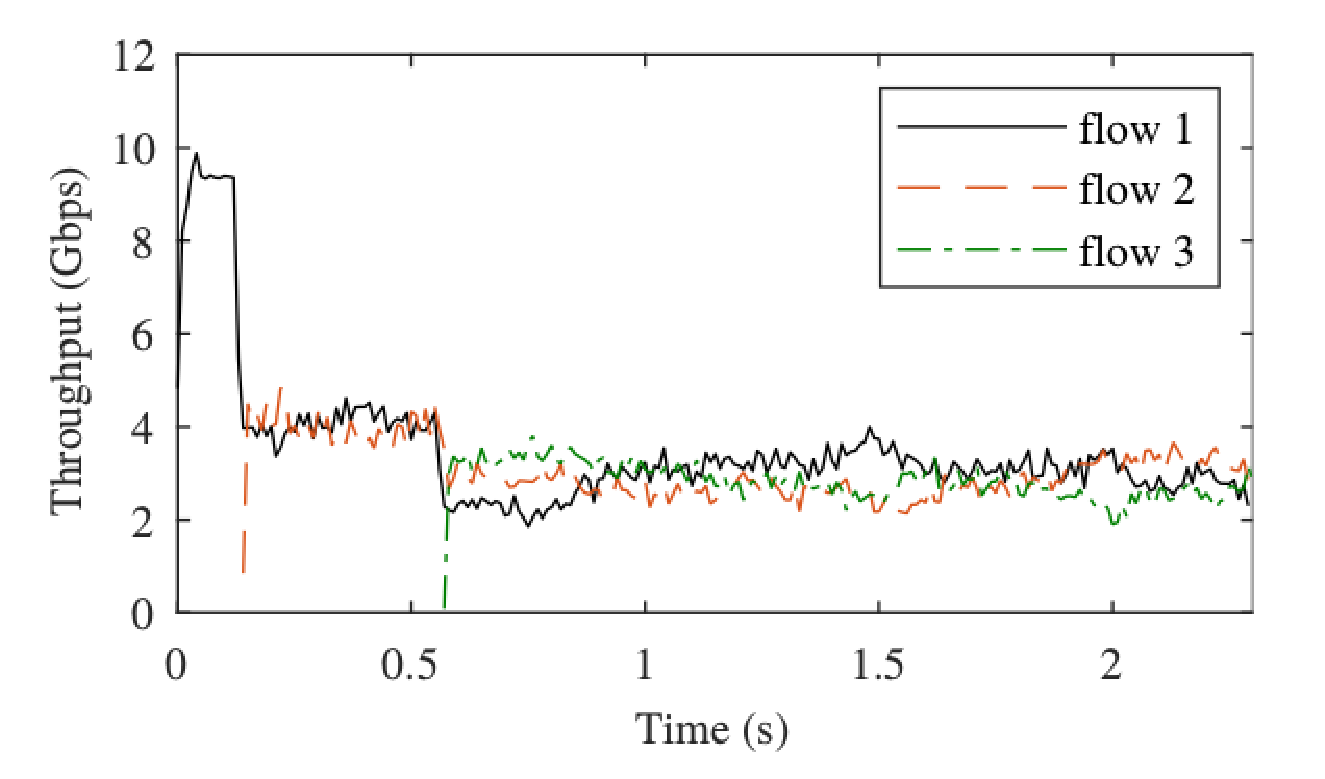
\includegraphics[width=4in]{cx4imp}
		\caption{DCQCN implementation of ConnectX-4 adapters}
		\label{fig:cx4imp}
	\end{center}
\end{figure}

Figure ~\ref{fig:ns3imp} shows the NS-3 simulation result of throughput with ConnectX-4 parameters.
\begin{figure}[h!]
	\begin{center}
		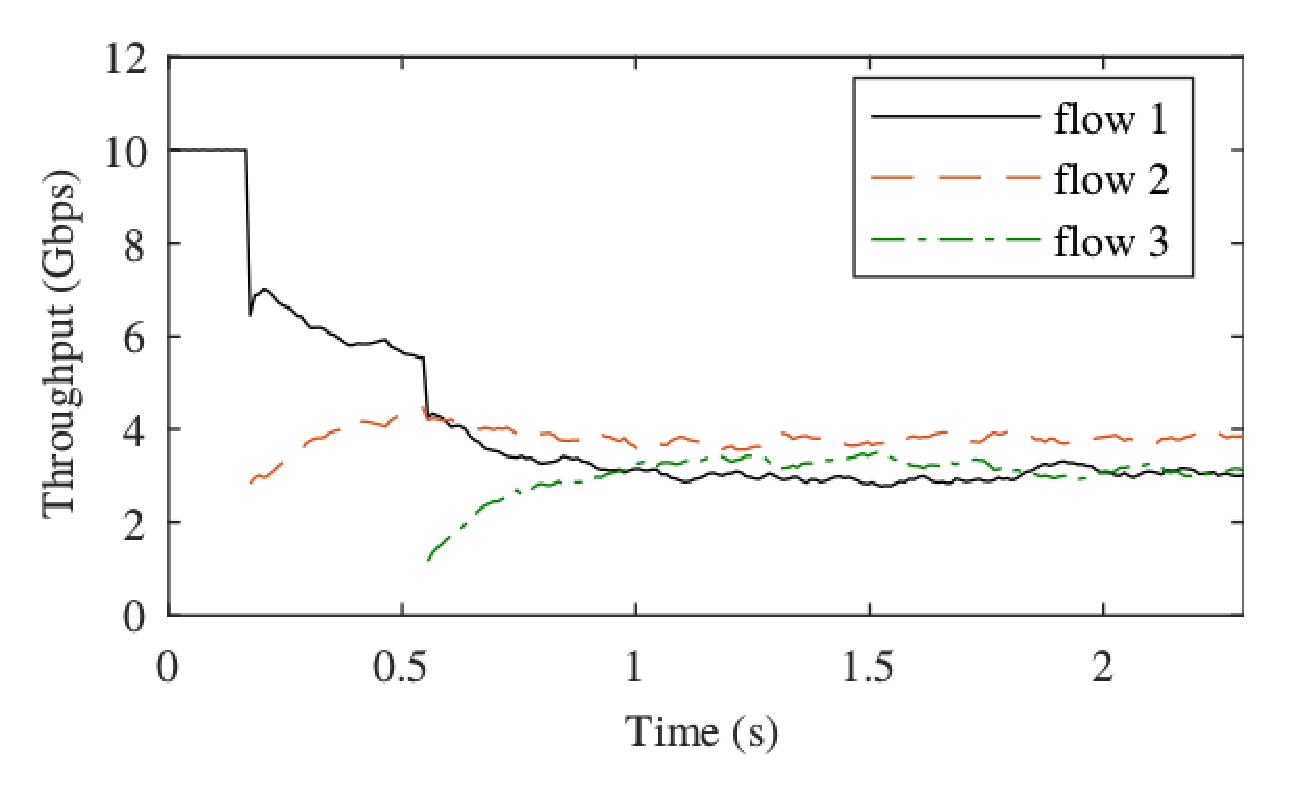
\includegraphics[width=4in]{ns3imp}
		\caption{NS-3 simulation with ConnectX-4 parameters}
		\label{fig:ns3imp}
	\end{center}
\end{figure}

That's different especially during the starting period in Figure ~\ref{fig:cx4imp} and Figure ~\ref{fig:ns3imp}.
ConnectX-4 should have made some improvements to the original DCQCN algorithm, especially at the beginning.
DCQCN starts at line rate but ConnectX-4 starts with speed reservation.

\newpage
\section{Improvements for DCQCN}

The key factor of DCQCN's failure is DCQCN's increase step, recovery speed and CNP supplies.
The information used are out of date for the growing scalability for data centers.
Those fixed increase steps, recovery speed and CNP intervals are not adaptive for large-scale traffic.
What we do is to find factors which actually influence the congestion and can predict the congestion level better.

Our work, DCQCN+ uses dynamic parameters to better analyze the congestion and therefore relieve it.
DCQCN never cares about the incast scale and thus uses fixed parameters to do the job.
That surely won't work for large-scale incast since the reaction and adjustments of sending rate are not very accurate.

DCQCN+ is designed to use the CNP period carried in CNPs and the flow rate to reflect the condition of the incast scale.
There are some remaining available fields to carry the period information of CNP.
Also, since larger flows are more probable to be marked with ECN, its possibility to trigger a CNP is larger.
Thus all congested flows can get similar rates and be balanced.

To be more specific, improvements are discussed from three points (Congestion Point, Notification Point and Reaction Point).

\subsection{Congestion Point}

This part remains almost the same.
What we can do at Congestion Point is really limited since CP is responsible for ECN marking.
The probability for ECN marks are very reasonable so we leave this part the same.

We also need to mention here that PFC is still enabled to ensure lossless feature of data centers.
Although our method can make sure that convergence can be reached in most cases, we can't ensure lossless feature at the starting burst
if PFC is disabled.

\subsection{Notification Point}

Receivers are in charge of generating CNPs.
This is the most important part of the algorithm.

At NP, two factors decide the CNP interval, the hardware ability to generate CNP and the demand for CNP at Reaction Point.
We hope to supply enough CNPs with shorter intervals for RP to properly adjust the sending rate.
At the same time, we don't want to cause other problems like CNP burst or CNP congestion if we set the interval which is too short.
Such problems may cause unnecessary bandwidth cost.
The ability of hardware may influence the minimal interval and demands for CNPs decide the maximal interval.
We prefer the maximal interval to relieve the possibility of bandwidth cost.

Once the flow rate collects enough information to decide the incast scale, the timer period should be decided.

\subsection{Reaction Point}

Here we first show the original DCQCN RP algorithm pseudocode in Figure ~\ref{fig:RPalg}.
\begin{figure}[h!]
	\begin{center}
		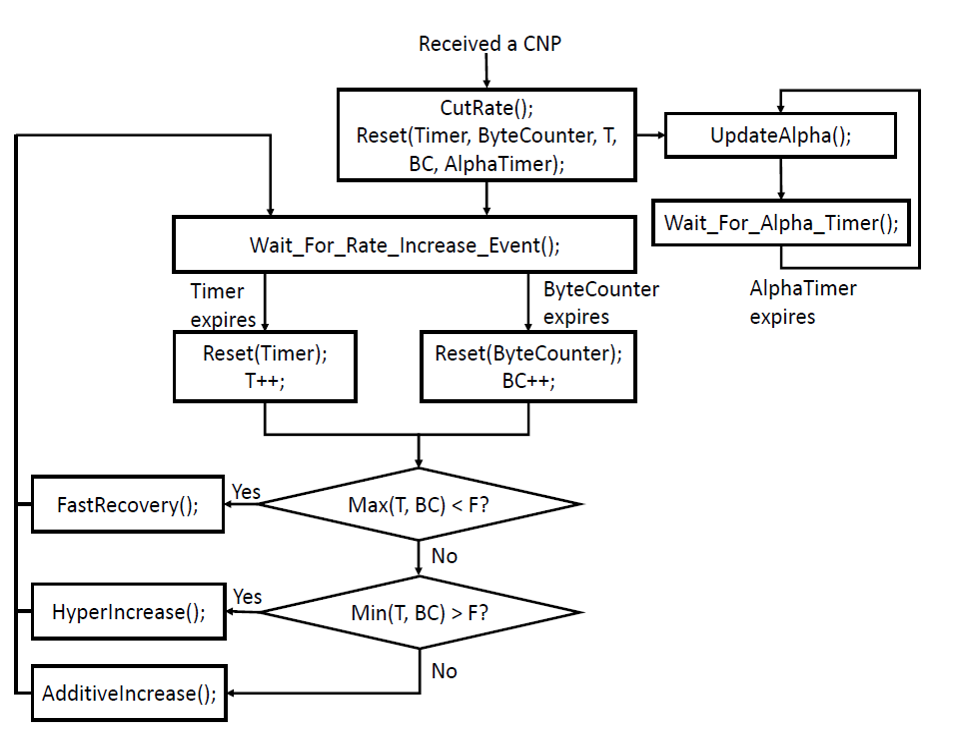
\includegraphics[width=6in]{RPalg}
		\caption{RP algorithm from DCQCN}
		\label{fig:RPalg}
	\end{center}
\end{figure}

We make some changes on the updates of parameters.

The reaction when receiving CNP is similar:
\[R_T=R_C\]
\[R_C=R_C(1-\alpha /2)\]
\[\alpha = (1-g)\alpha + g\]

Here $\alpha$ is a reduction factor, actually indicates the congestion level at the CP.
$R_C$ denotes current rate and $R_T$ denotes target rate.
$g$ is a parameter to estimate the congestion level.

Instead of DCQCN's fixed rate increase timer $K=55\mu s$, we make it flexible:
\[K=\lambda max(\tau, \frac{MTU}{R_C})\]
where $MTU$ denotes Maximal Transmit Unit and $\tau$ denotes CNP interval.

Here we remove the byte counter and add the rate increase counter.
When the rate increase counter times out, the state S increases 1.

The fast recovery scheme remains the same when $S$ is less than the threshold $F = 5$:
\[R_C=\frac{R_C+R_T}{2}\]

When $F<S<4F$,
\[R_T=R_T+ min(\frac{1}{10}R_C,\frac{1}{100}R_l)\]
\[R_C=\frac{R_C+R_T}{2}\]
where $R_l$ is a ratio used to bound the increase step for small incast cases.

When $S>4F$, Hyper Increase is applied,
\[R_T=R_T+min(R_C, \frac{S-4F}{100}R_l)\]
\[R_C=\frac{R_C+R_T}{2}\]

Additionally, when $\alpha$ timer runs out,
\[\alpha=(1-g)\alpha\]

To be more clear, we get Figure ~\ref{fig:RPalgplus} to show our new RP algorithm.
\begin{figure}[h!]
	\begin{center}
		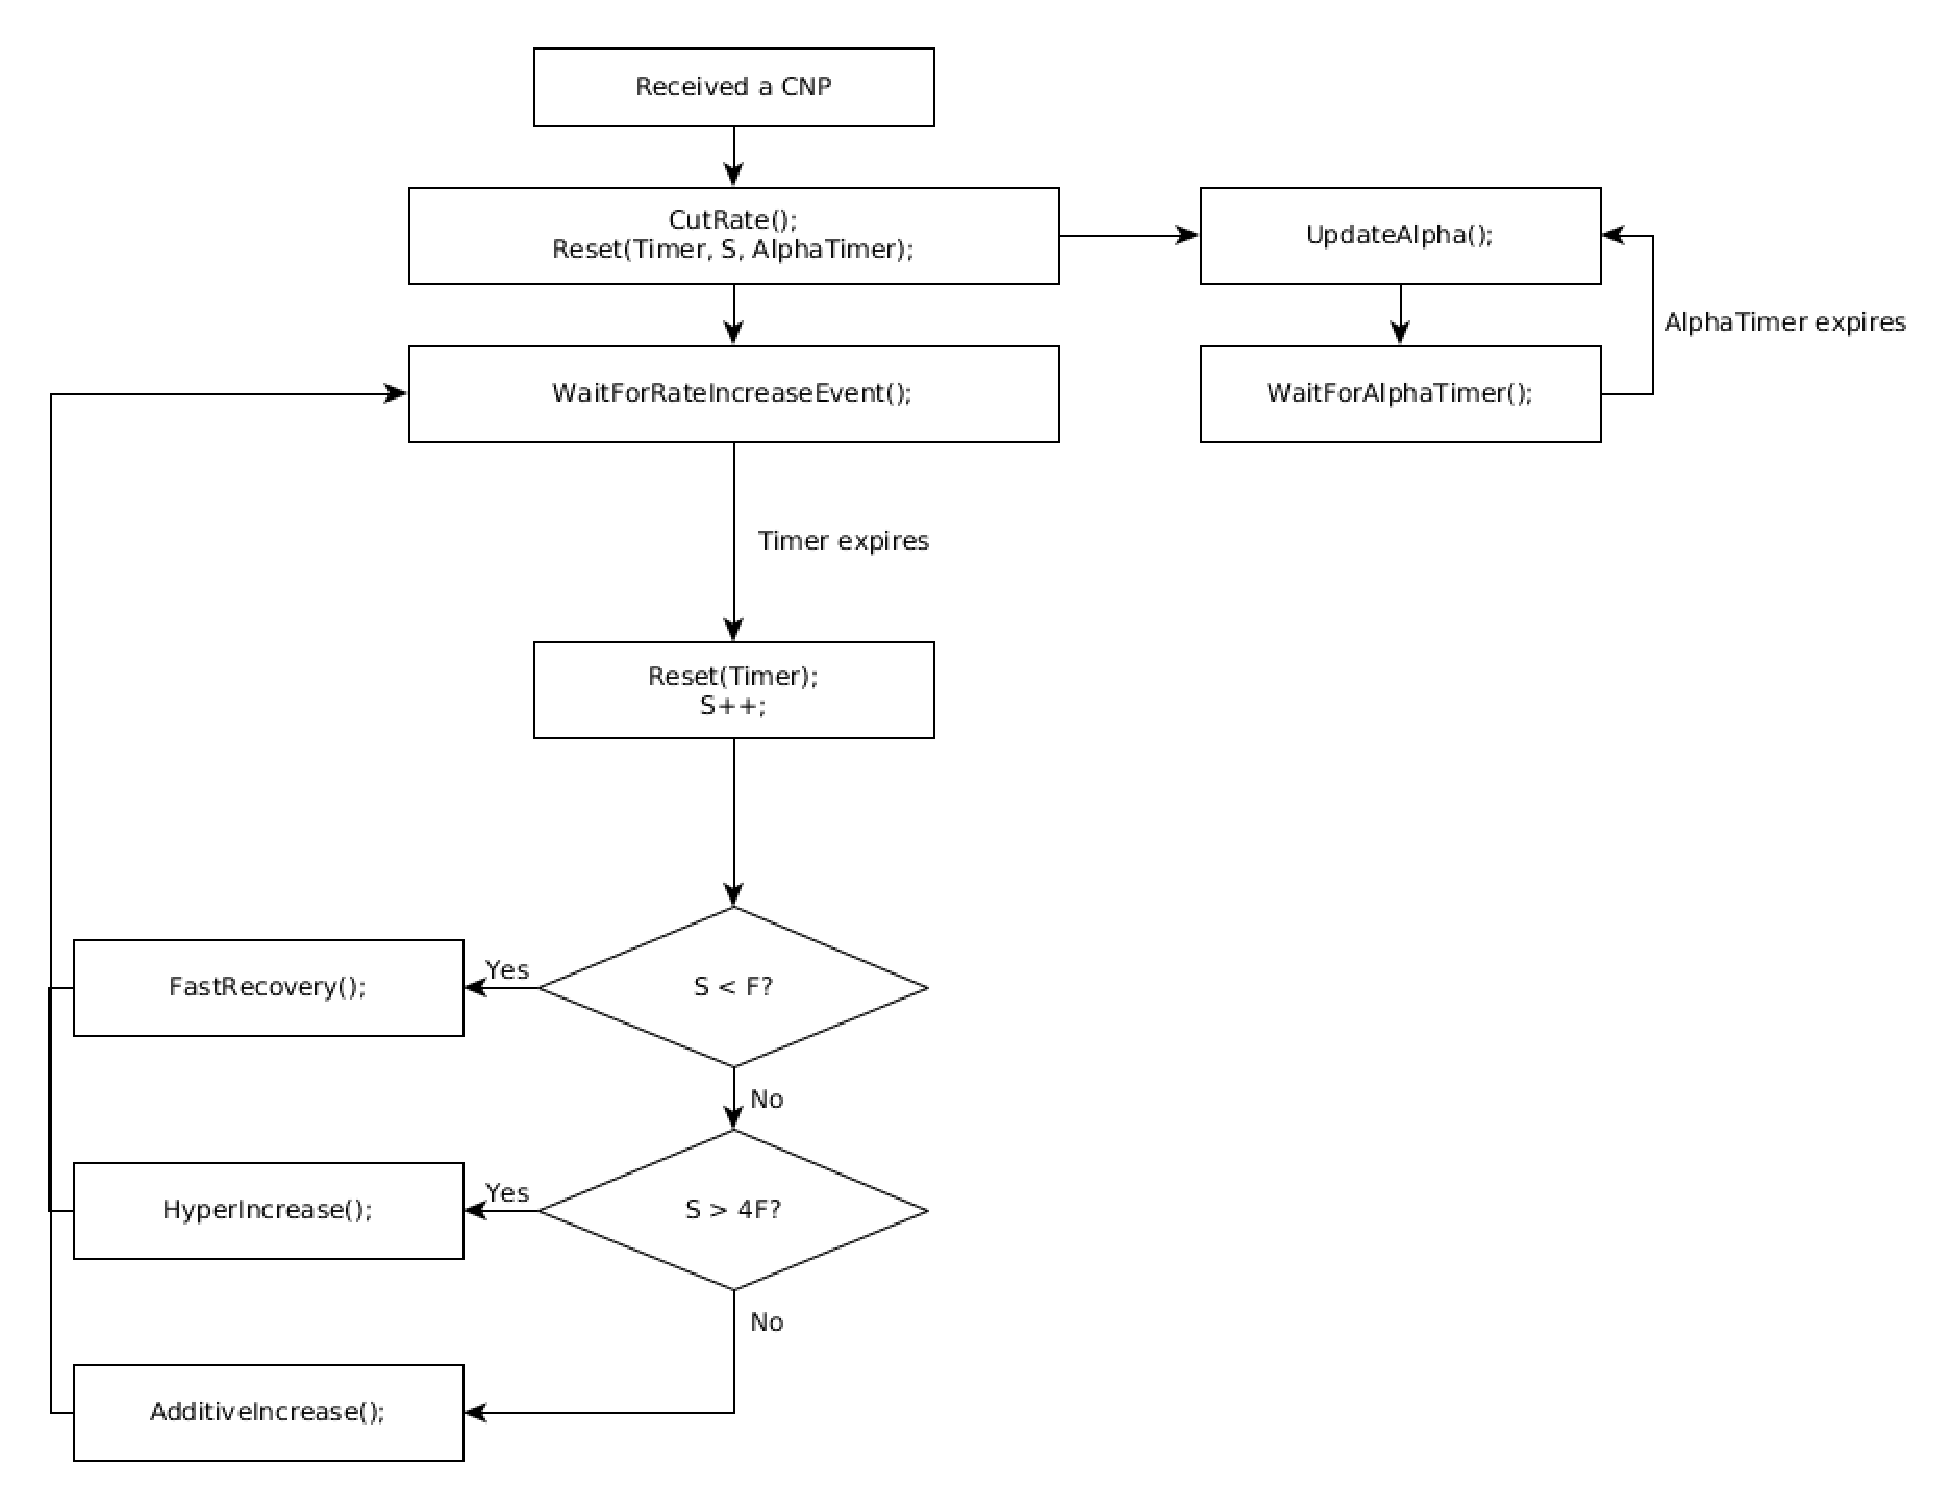
\includegraphics[width=6in]{RPalgplus}
		\caption{RP algorithm from DCQCN+}
		\label{fig:RPalgplus}
	\end{center}
\end{figure}

We can see a lot of changes to make the algorithm better.
Such dynamic adjustments of parameters greatly improve the buffer estimation in advance and drain the congestion fast
to maintain the buffer queue length low.

\newpage
\section{Implementation}

We set up the testbed of testing for DCQCN+ on Mellanox SN2700 switch and 9 Ubuntu servers with ConnectX-4 adapter cards.
Mellanox SN2700 provides the most predictable,
highest density 100GbE switching platform for the growing demands of today's data centers,
which can easily satisfy our experiment environment for over 400 flows at a time.
ConnectX-4 dual-port adapter cards with Virtual Protocol Interconnect (VPI) support 100Gb/s InfiniBand and 100Gb/s Ethernet connectivity.
All the features including RoCE v2 \cite{RoCEv2}, PFC and ECN are supported on Mellanox SN2700 and ConnectX-4 adapter card.

To generate enough number of flows for our experiment, the topology is shown in Figure ~\ref{fig:Topology}.
Each machine can create several and even tens of flows simultaneously.

\begin{figure}[h!]
	\begin{center}
		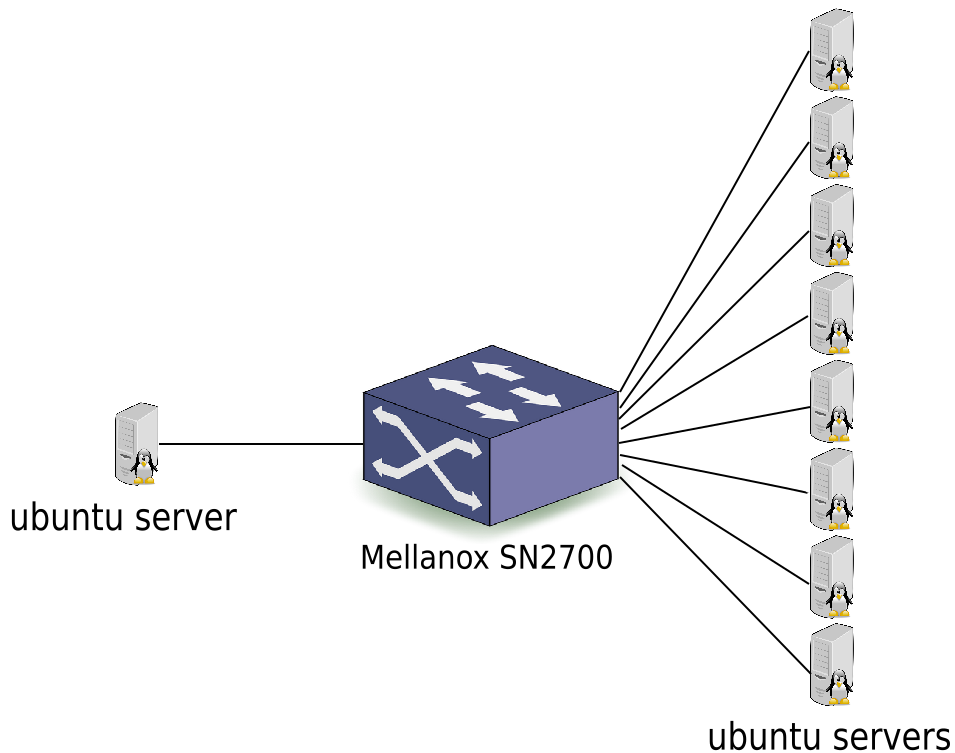
\includegraphics[width=3in]{Topology}
		\caption{Topology for multi-flow tests}
		\label{fig:Topology}
	\end{center}
\end{figure}

To be clear in Figure ~\ref{fig:Topology},
we regard the server on the left (which is the receiver) as S0 and the servers on the right (which are senders) as S1 to S8.
All the servers are configured into the same virtual local area network (VLAN) so that we can construct an incast traffic inside the network.

\subsection{Switch Configuration}

Mellanox SN2700 has provided a lot of interfaces for users.
Among them, we need to configure VLAN, PFC, ECN and buffer size to make things work.

All the configurations are done according to the manual.

\subsubsection{VLAN}
The whole experiment environment should be separated from outside traffic including SSH connection and SFTP file transmission.
VLAN is thus needed to create a separate topology.

Switch need to enable the VLAN feature and include all machines in the same VLAN session.
This includes some work on distinguishing ports.

\subsubsection{Port mirroring}

We try to collect the InfiniBand traffic from
receiver end thus we don't need to process the received information from all different senders.
However such method doesn't work because we can't sniffer the InfiniBand traffic from the receiver side.

Mirroring is also configured as sessions in switches.
In our experiment, we configure the session's input as the receiver and the output as another vacant machine in the same rack.
After flows are started, we start Tcpdump on the mirror session's output machine to capture packets.

Such a method can deal with small-scale incast but not large-scale ones.
Even an enlarged buffer size for Tcpdump can't handle the amount of traffic in large-scale incasts.

\subsubsection{PFC}
PFC is needed because what we want is a lossless network which is a must for data center networks.
PFC makes receiver to send PAUSE frame to sender where sending ratio is limited upon received PAUSE.
Default PFC configuration contains 8 priority classes and we only have 2 used here.
The mapping is mentioned in the following subsection about ECN.

\subsubsection{ECN}
ECN priority is configured to make CNP function well. Higher priority is needed for a higher traffic class.
Inside our experiments, there are mostly two classes of traffic. RDMA traffic is in traffic class 3 and should be mapped to switch priority 3.
Other traffic like TCP is in traffic class 0 and should be mapped to switch priority 0.
The reason is that the traffic for setting up a flow shouldn't be blocked. If we don't set the priority difference, the flow setup traffic for a flow
is blocked when there are really a large number of flows. The flow setup period should use higher priority so that more flows can be created.
About this point, we explain it in later sections.
And the probability to make an ECN mark should be configured the same as mentioned in DCQCN \cite{dcqcn}.

\subsubsection{Buffer}
About the buffer size, we don't need to be very specific. The maximal buffer size inside Mellanox 2700N switch is 5.1MB.
One important factor to be considered is the buffer usage during the experiment process.
When a lot of flows are created, there must be a burst of packets in the receiver buffer at the beginning.
After a short period of reaction time, the buffer usage should go down because the senders are limited by the switch based on flows.
In the results, what we are hoping to see is that the beginning of the buffer is large but after the short reaction time, the buffer is low.
Thus the buffer here is only to handle the burst at the beginning.

\subsubsection{Additional Configurations}
To make things clear, we need to cut unnecessary parts of traffic.

We obviously don't contain loops inside our topology so that the spanning tree protocol is removed from the switch.

The interface speed is set to 100Gbps when testing the hardware ability to generate CNP.
For other most experiments, interface speed is configured as 10Gbps (the reason is explained in later sections).

\subsection{NIC Configuration}
At the very beginning, we need to install Mellanox OFED (driver for ConnectX-4) for every server.

After that, we have several steps (most corresponds with the upper switch configurations):
\begin{enumerate}
	\item Enable PFC and set up the priority.
	\item Enable ECN for both InfiniBand traffic and TCP traffic.
	\item Set CNP priority and DSCP priority.
	\item Set priority for RDMA traffic.
	\item Open sniffer for Tcpdump \cite{Tcpdump} to capture InfiniBand packets.
\end{enumerate}

To make all the things easier, I write Python scripts to make things automatic.
With Paramiko, we can do the remote command execution work.
I can list all the IPs needed to be configured and use Paramiko to configure them all.

The only thing tough in this is to execute a command with root.
And I use ''sh'' to get the root-necessary command executed just like this:
\begin{lstlisting}
sudo sh -c \'echo "0" > /sys/class/net/p4p2/ecn/roce_np/min_time_between_cnps\'
\end{lstlisting}

Directly executing commands on remote machines using Paramiko doesn't work because the ''sudo'' is actually running part of
the user-level commands.
''sh'' indicates the exact necessary tool needed for execution so ''sudo sh'' knows to execute with shell clearly.

\subsection{Experiment Process}

The general idea is creating an incast and observe the congestion point.
To be more specific, we are generating flows from S1~S8 (tens of flows from each) and observe the bandwidth tendency, latency and buffer usage.

However, before all of that, the first experiment is to test the CNP generation speed for ConnectX-4 and ConnectX-5. 

\subsection{Ability to Generate CNP}

All NIC has limited ability. For ConnectX-4 and ConnectX-5, we hope to figure out the exact ability to do this so that we can adjust the DCQCN efficiently.

The topology is simple. Two servers are connected to the switch, one as the sender and one as the receiver.
For the receiver side, the interface speed is set to 10Gbps. The sender side has an interface speed of 100Gbps.
Thus the congestion surely exists and we use Tcpdump to capture the packets during a short period of time.

Among the packets captured inside the Pcap file, we filter the traffic with the right direction and right IP addresses out.
According to the timestamps, we can know something about the ability of ConnectX-4 and ConnectX-5.

\subsection{Bandwidth Testing}

Now the topology is the one shown in Figure ~\ref{fig:Topology}.
We use the command ib\_send\_bw to start flows.

Bandwidth testing needs several steps:
\begin{enumerate}
	\item Refresh machine states.
	\item Time synchronization for all servers.
	\item Start Tcpdump simultaneously on S1 to S8.
	\item Start ib\_send\_bw server on S0.
	\item Start ib\_send\_bw clients on S1 to S8.
	\item Send Pcap files to local.
	\item Parse Pcap files.
	\item Use parsed results to draw bandwidth figure.
\end{enumerate}

The overall tests are done by scripts of many languages including Python, C, Bash, Awk and Gnuplot.

Let me describe the above steps one by one.

\subsubsection{State Refresh}

Because we start a large number of flows on each machine, the command of ib\_send\_bw may fail to complete correctly, leaving
some processes continuing during the stages. We need to refresh the states for machines.

To kill the processes running from the last experiment, we use the command ''pkill -f'' to kill processes with the label of ''ib\_send''.

\subsubsection{Time Synchronization}
We use Network Time Protocol (NTP) to synchronize the time for S0 to S8.
The accuracy for NTP is about 0.01ms so that should work for servers on a rack.
Choosing a server inside the same rack, we set up an NTP server on it.

Then we use Python Paramiko to execute the NTP command on S0~S8 for time synchronization with the NTP server.

Here we need to claim a fact that the receiver side can't tolerate the number of packets we need to actually generate a bandwidth figure.
Even an increased size of Tcpdump buffer can't hold the traffic of even 1 second which is obviously not enough to analyze the bandwidth tendency.
Thus we are running Tcpdump on each machine which can last for approximately 10 seconds.
With time synchronized, we can analyze packets on different machines with timestamps correct.

\subsubsection{Tcpdump Start}
Python Paramiko is still the tool used for remote command execution.

Different from normal Tcpdump, we need to specify several parameters here.
''-B 900000'' parameter is needed to increase the buffer size of Tcpdump.
''-s 60'' parameter is to capture only the first 60 bytes which contains just the packet headers.

It's hard to estimate the capturing time needed, but we can limit the packet counter of Tcpdump (which uses ''-c'').
Thus the file size is shrunk and it saves time for file transmission.

\subsubsection{ib\_send\_bw Server Client Starter}

This step contains concatenation work.
What we are doing is to accept parameters from the command line execution of the program.
This contains the concatenation of mark ''\&'' and other strings.
''\&'' is used for simultaneous command execution. Linux System usually has the ability to run over 1000 processes simultaneously.

The repeated part is like this:
\begin{lstlisting}
ib_send_bw -S 3 -x 5 -d mlx5_1 192.168.33.85 -D 80 -p 
\end{lstlisting}
We need to repeat such lines with combined port number and ''\&''.
Such a concatenation will last very long but still tolerable by the machines to execute.

Especially for the receiver (S1), the command may repeat for hundreds of times but the multiprocess upper bound
is over 1000.

Luckily string operations are easy for Python.
I'm actually recording the same parts of the commands and adding loops with transformed string from numbers.

The command I use is like this:
\begin{lstlisting}
ib_send_bw -S 3 -x 5 -d mlx5_1 192.168.33.85 -D 80 -p 10010
\end{lstlisting}

About the detailed information about the commands, we have several specific options set.
The option ''-R'' is for RDMA connection setup. However, we find that using RDMA traffic for a flow start causes
the traffic congested with other already-started flows. Thus we may fail to start a lot of flows at the same time.
So in real experiments, we are not using the option.

The option ''-S 3'' means the priority class for RDMA traffic. This can also be set for RoCEv2 protocol.
We add it here just to be sure that the traffic class priority is working.

The option ''-x'' denotes the device ID we are using, which can be fetched through the command ''show\_gids''.
This displays the ROCE version we are using and the corresponding device ID and destination IP.
''show\_gids'' is only needed once for each machine so that it's not actually included as part of the automation tool.

The option ''-d'' denotes the network devices used for the execution which is mlx5\_1 for our machines.

The option ''-D'' shows the lasting time of our experiment. It counts in seconds of the continuous sending procedure.
In our experiment, it's usually 60 or 80 which shows almost a complete tendency of the bandwidth and flows.

The option ''-p'' is responsible for separating flows. In our experiment, we hope to create multiple flows from one machine.
The number could be tens and even reach 90 so we need to use port number to start different flows.
The actual implementation of port allocation is like this: 

We are taking parameters of machine number and flow number of each machine at the beginning of the overall scripts.
Assume that they are $m$ and $n$.
All port number for flows starts from 10011. There is a continuous range from 10011 to $10010+m\times n$ for port numbers.
The first machine takes the position of port number like 10011, $10011+m$, ..., $10011+m\times(n-1)$.
To be more general, the $i_{th}$ flow on the $j_{th}$ machine (where $i=1,2,...,n$ and $j=1,2,...,m$) has the port number of
$10010+i+m\times(j-1)$.
Thus all the port numbers don't collide with each other. This makes later steps easier to process.
Those are mentioned in later sections.

\subsubsection{File Transmission}
To be clear, we are running experiments on 9 machines.
Besides that, we have a middle machine with accounts to log in, making the machines more secure.
And we have a local machine to process the results we get. We are using a local machine to do this because
we hope to keep the experiment machines clean and fewer new tools should be used there.
I use Python Paramiko for remote login and file transmission.
A tough point is that all file location should be absolute locations but that's OK since the amount needed is not very large.

Thus the file transmission has two parts. The first step would be sending Pcap files from experiment machines to the middle machine.
The second would be transmitting the files from the middle machine to the local machine.

\subsubsection{Pcap Parsing}
This contains several steps. We can't make sure that this is the easiest way to process these packets but it works fine.
\begin{enumerate}
	\item Transform Pcap files to plain text.
	\item Filter the packets to get the traffic with the receiver we want.
	\item Divide the packets from all different flows in the same machine.
	\item Collect number of packets in every millisecond.
	\item Transform timestamps to relative time starting from the beginning of the flows.
	\item Add counts of zeros for those milliseconds which contains no packets.
\end{enumerate}

For step 1, I use the command of Tcpdump with the option of ''-r'' which means reading.
With options ''-rrrr'' and ''-nnq'' we transfer the Pcap file into plain text with 8 terms.
Among them, we have the timestamp, source IP, source port, destination IP and destination port.
Thus we can approximately calculate the bandwidth from such information.

The complete command used is here:
\begin{lstlisting}
s= ['tcpdump -r /home/yangyuchen/Research/automation/multiflow/'+str(i)+'.pcap -s 60 -i p4p2 -tttt -nnq > /home/yangyuchen/Research/automation/multiflow/'+str(i)+'.txt']
\end{lstlisting}

For step 2, I use Awk to do the filtering. By limiting the receiver as the only host we regard as an incast receiver, we get all the receiver IP (which is the
$6^{th}$ term of the plaintext) out of all possible flow receivers.

The complete command used is here:
\begin{lstlisting}
s=['awk \'{ if (index($6,"192.168.33.85")==1) { print $0 } }\' /home/yangyuchen/Research/automation/multiflow/'+str(i)+'.txt > /home/yangyuchen/Research/automation/multiflow/'+str(i)+'_data.txt']
\end{lstlisting}

For step 3, we can only divide all the flows on the same machine using the ports.
TCP and InfiniBand have its unique port forwarding methods which would surely dismiss the ports I set for them in the ''ib\_send'' commands.
To separate all these flows, I write a C++ program to do the filtering work, collecting all the different port numbers and raise flags for new port numbers.
Each new port number starts a new file for collection, containing the packets of a single flow.
The file names are carefully calculated.
Suppose we have $m$ machines and each starts $n$ flows, then the numbering of the file names are similar to the one previously mentioned in port numbering.
The only difference is that port numbers start from 10010 and the file names start from 85 (which is the machine index in our testbed).

For step 4, I specifically count the digits in every line (which contains a packet) of the plain text. Thus I can make sure which digits represent the condition
of the timestamps. 
Then I decide in plain text which exact digit decides the millisecond and which digit is the starting point of the timestamp.
To decide the number of packets in one millisecond, we can find the ones with a sharing first 3 digits after the decimal point in the timestamp.
To do the filtering and counting work, we have an easy command-line tool which is ''cut''.
Using the option of ''-c'', we can have a count on the packet number with the same timestamp till millisecond digit.
Therefore, we print the timestamps and the packet numbers. (which has two columns and therefore can be drawn into a figure.

The command used is here:
\begin{lstlisting}
s=['cut -c 1-12 /home/yangyuchen/Research/automation/multiflow/'+str(i)+'_divideddata.txt | awk \'{print $1}\' | sort | uniq -c  | awk \'{print $2 " " $1}\' > /home/yangyuchen/Research/automation/multiflow/'+str(i)+'_packets_count.txt']
\end{lstlisting}


Step 5 and step 6 are relatively easy. 
Record the earliest packet occurs and do subtractions.
Then we need to add zeroes for those milliseconds which contains no packet to make the figure fluent and complete.

All this part is using C language and these parts are running on local machines.
Step 5 includes reading files and rewriting to a new file with the same index number but different header in file name.
Step 6 is simply some traversing over the whole timestamps.

\subsubsection{Figure Plotting}

Here we use the tool of Gnuplot, which is a practical plotting tool under Linux systems.

We have figured out the timeline and packet count for each millisecond before.
For most packets, they have the same size of 1KB which is fixed by the command ''ib\_send''.
Thus we can indicate the bandwidth through packet count of each millisecond.

Gnuplot can take the number of machines and flow number of each machine as parameters.
When plotting, we need to choose data from different files with the names in sequence.

Because we don't know the number of flows we are drawing, we can't list the exact colors of lines and points.
Here I simply use numbers to choose colors from Gnuplot's color library.

Most figures shown in the results are drawn using Gnuplot.
To be more clear about the coloring condition, we can take a look at Figure ~\ref{fig:3_20_0}.

We can also display a simple example of how we plot the figures using Gnuplot.
\begin{lstlisting}
set title "packets/millisec"
set xlabel "reltime"
set ylabel "packets count"

set style line 1 linecolor rgb "#000000" lw 1

j=ARG1
k=ARG2
plot for [i=86:86+j*k-1] '/home/yangyuchen/Research/automation/multiflow/'.i.'_reltime_count.txt' using 1:2 title ''.i with line ls i-85

set terminal png font "/Library/Fonts/Arial.ttf" size 1600,900
set output "/home/yangyuchen/Research/automation/multiflow/packets_count.png"

replot
\end{lstlisting}

Here sadly we also have to use absolute file locations.

Those ''*\_reltime\_count.txt'' are stored with two columns with time and packet number respectively.
And the line colors are displayed with $i-85$ which makes every color starting from 1.

With the title and labels all set, we also need to set the output format as PNG to make it readable by all systems.
The original picture was super detailed with a pixel resolution of $1600*900$.
Thus we can see every detail of bandwidth changes, especially at the starting period to make algorithm design easier.

\subsection{Latency and Buffer Usage}

Most steps are similar to the last subsection about bandwidth testing.
We are doing this part because as the flow number increases bandwidth collecting is super time-consuming.
Sometimes this part may last hours and the figure we get is unclear and lines overlap each other.

Latency and buffer usage can reveal the effect of convergence more effectively.
For latency, I'm using ''ib\_send\_lat'' on each machine which provides average latency and extreme latency during a time period.
What I collect is simply the average latency which is shown in Table ~\ref{tab:default} and Table ~\ref{tab:improved}.

The command I'm using is listed here.
\begin{lstlisting}
ib_send_lat -S 3 -x 5 -d mlx5_1 192.168.33.85 -D 80 -p 10010
\end{lstlisting}

With filtered returning messages, I can gain information from the screen output.
The output should include 8 lines with each describing the result from 1 machine.
I collect the results and find some rules inside.

About buffer usages, I collect manually from interfaces provided in Mellanox switches.
I collect buffer information every 10 seconds to get them collected in Table ~\ref{tab:default} and Table ~\ref{tab:improved}.
All the flows last for 80 seconds and I start collecting from the $10_{th}$ second and manually read the buffer every 10 seconds.
Altogether I collect buffer usage information for 7 times which is sufficient for us to analyze the condition.

\newpage
\section{Results}

\subsection{NIC Ability to Generate CNPs}
We test the ability to generate CNPs for both ConnectX-4 and ConnectX-5 NICs.

The experiment topology is really simple.
Two hosts are connected to the Mellanox SN2700 switch, with the interface speed configured to 10Gbps and 100Gbps respectively.
The 100Gbps one then sends continuous InfiniBand traffic to the 10Gbps one.
When the switch is correctly configured with PFC and ECN enabled, we can find a burst of CNPs in a short period of time.

CNP can be distinguished by filtering the OP code of InfiniBand header which is 129.
Then I find a period of continuous CNPs and can get the approximate interval between CNPs.
With the parameter of CNP interval (min\_time\_between\_cnps) is set to 0, the results collected are just what we want.

Figure ~\ref{fig:CNPint} shows the interval of continuous CNPs under ConnectX-4 adapters.

\begin{figure}[h!]
	\begin{center}
		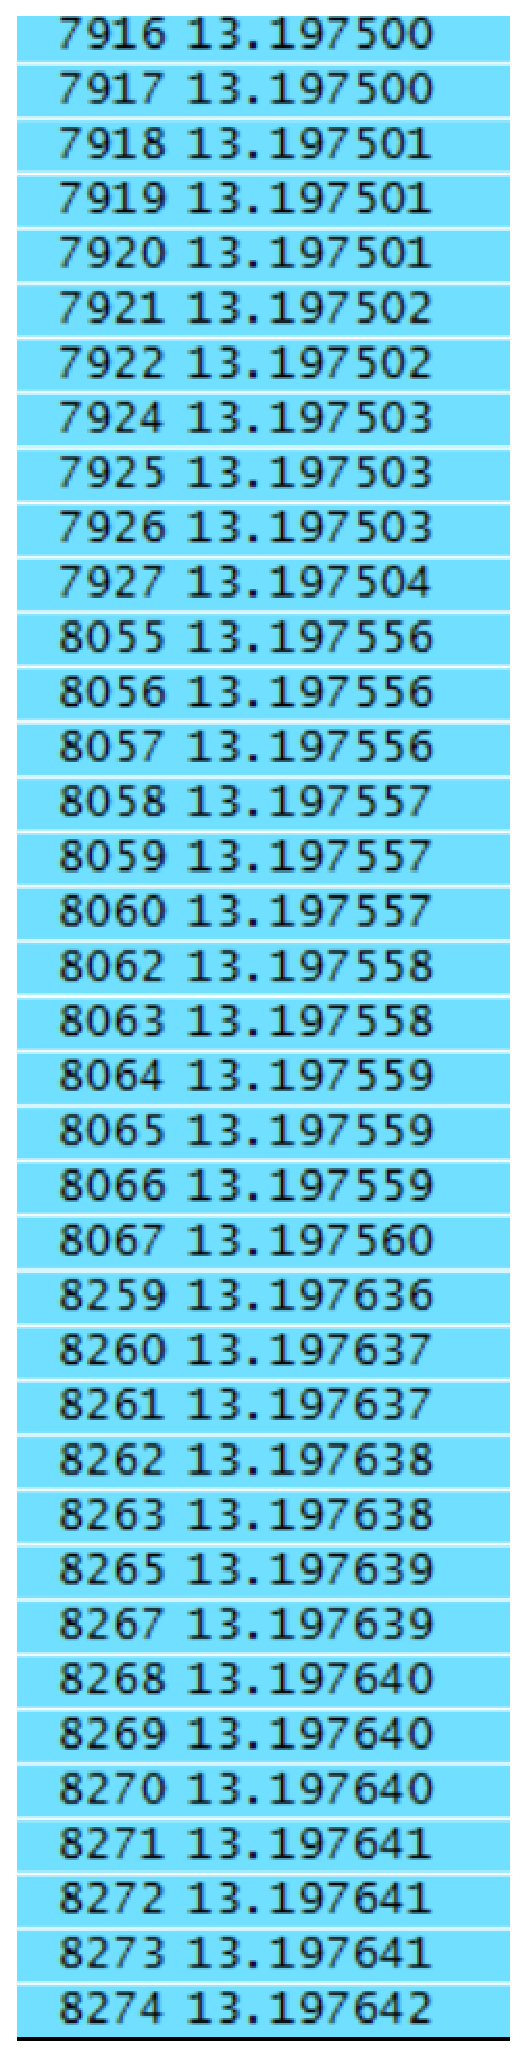
\includegraphics[width=1in]{CNPint}
		\caption{CNP interval test}
		\label{fig:CNPint}
	\end{center}
\end{figure}

The first column marks the packet number (those ommitted are not CNPs) and the second column includes timestamps in seconds.

Tcpdump with RDMA packet sniffer on can capture enough packets to generate the results.
ConnectX-4 NIC can generate 1 packet per microsecond.
ConnectX-5 NIC can generate 3 packets per microsecond.
We can find some small improvements in hardware ability between the NICs of the two generation.
Both are capable of our DCQCN+ algorithm.

\subsection{Bandwidth Condition for Small-Scale Incast}
In the beginning, we are not sure about our switch's ability, so we conducted some small-scale incast to test the switch and our configurations.
This can be called a duplicate of the original DCQCN.
The topologies are similar to Figure ~\ref{fig:Topology} but the number of receiver hosts varies.
All the interface speeds are set to 10Gbps.

Here are the examples of several experiments.

In Figure ~\ref{fig:2on1_1}, it's a 2:1 incast with flows from 2 machines.

\begin{figure}[h!]
	\begin{center}
		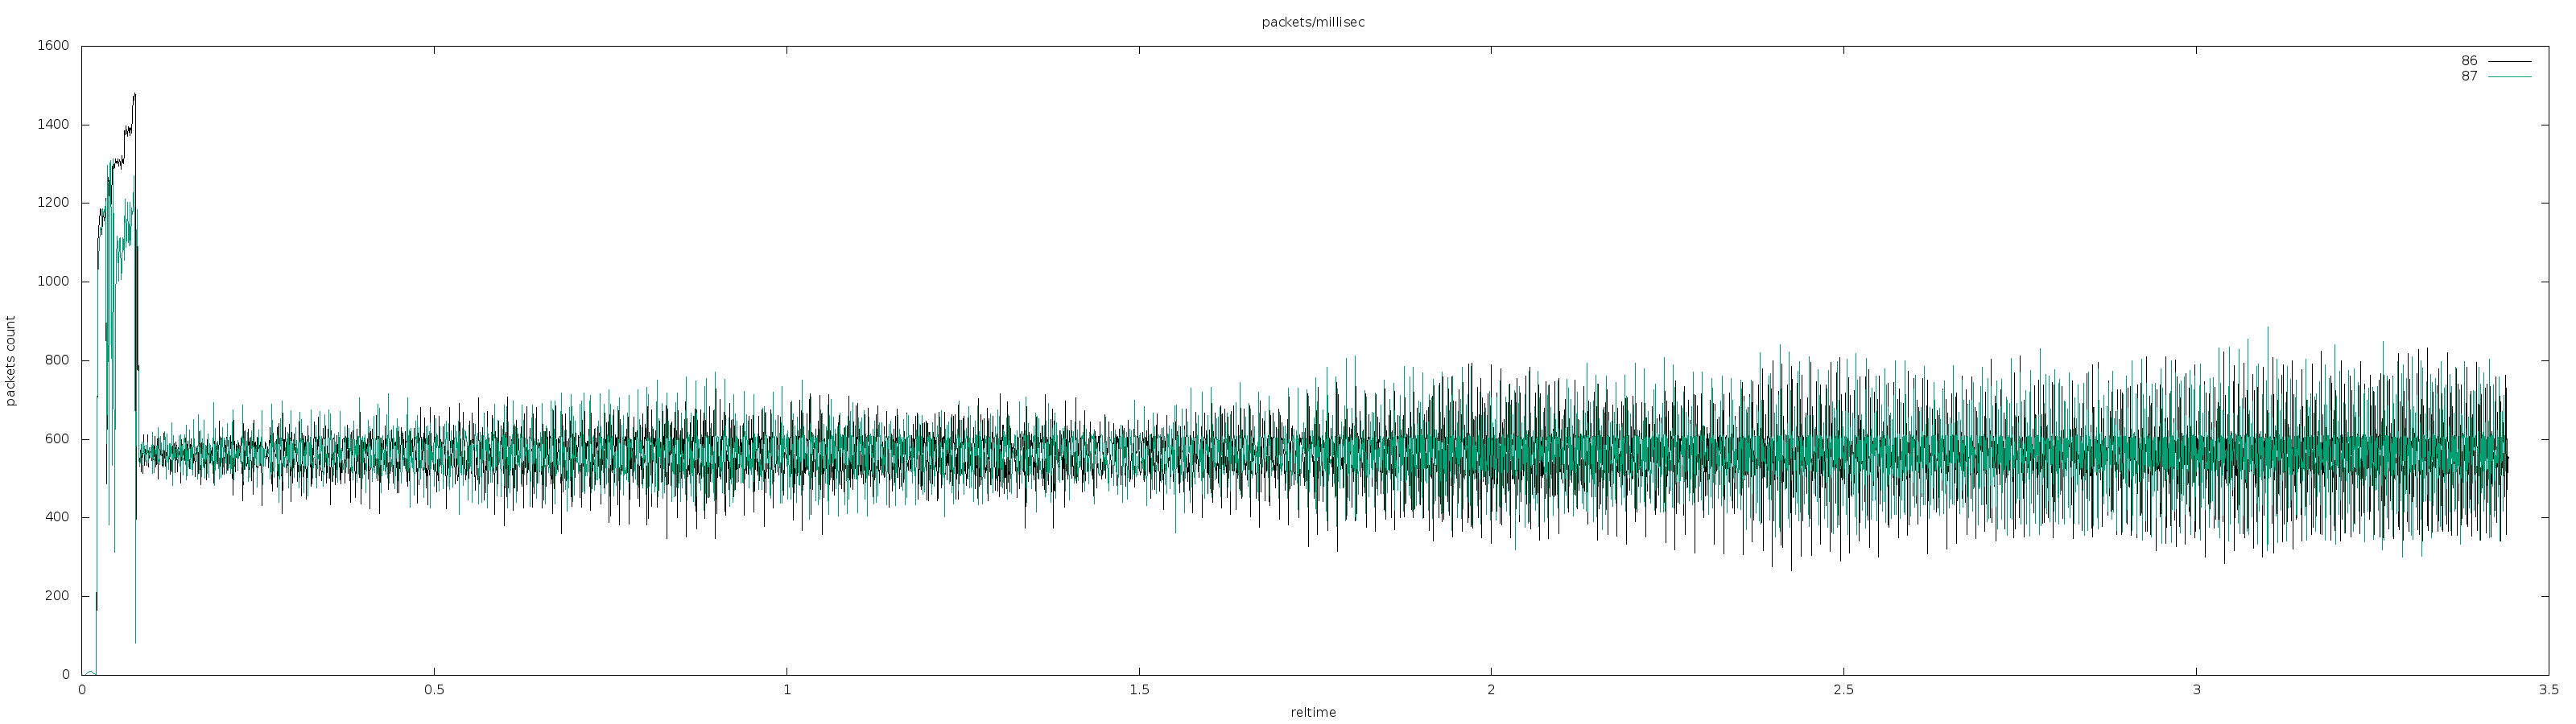
\includegraphics[width=6in]{2on1_1}
		\caption{2:1 incast bandwidth}
		\label{fig:2on1_1}
	\end{center}
\end{figure}

We can see, at the beginning of the flows, there's a line-rate start and the speed swiftly climbs to over 10Gbps.
After that, CNPs start working and both flows begin to limit sending rate and later within 0.5s, their speeds converge about
600 packets per millisecond, which is about 5Gbps.

In Figure ~\ref{fig:10on1_1}, it's a 10:1 incast with 10 flows coming from 10 hosts.

\begin{figure}[h!]
	\begin{center}
		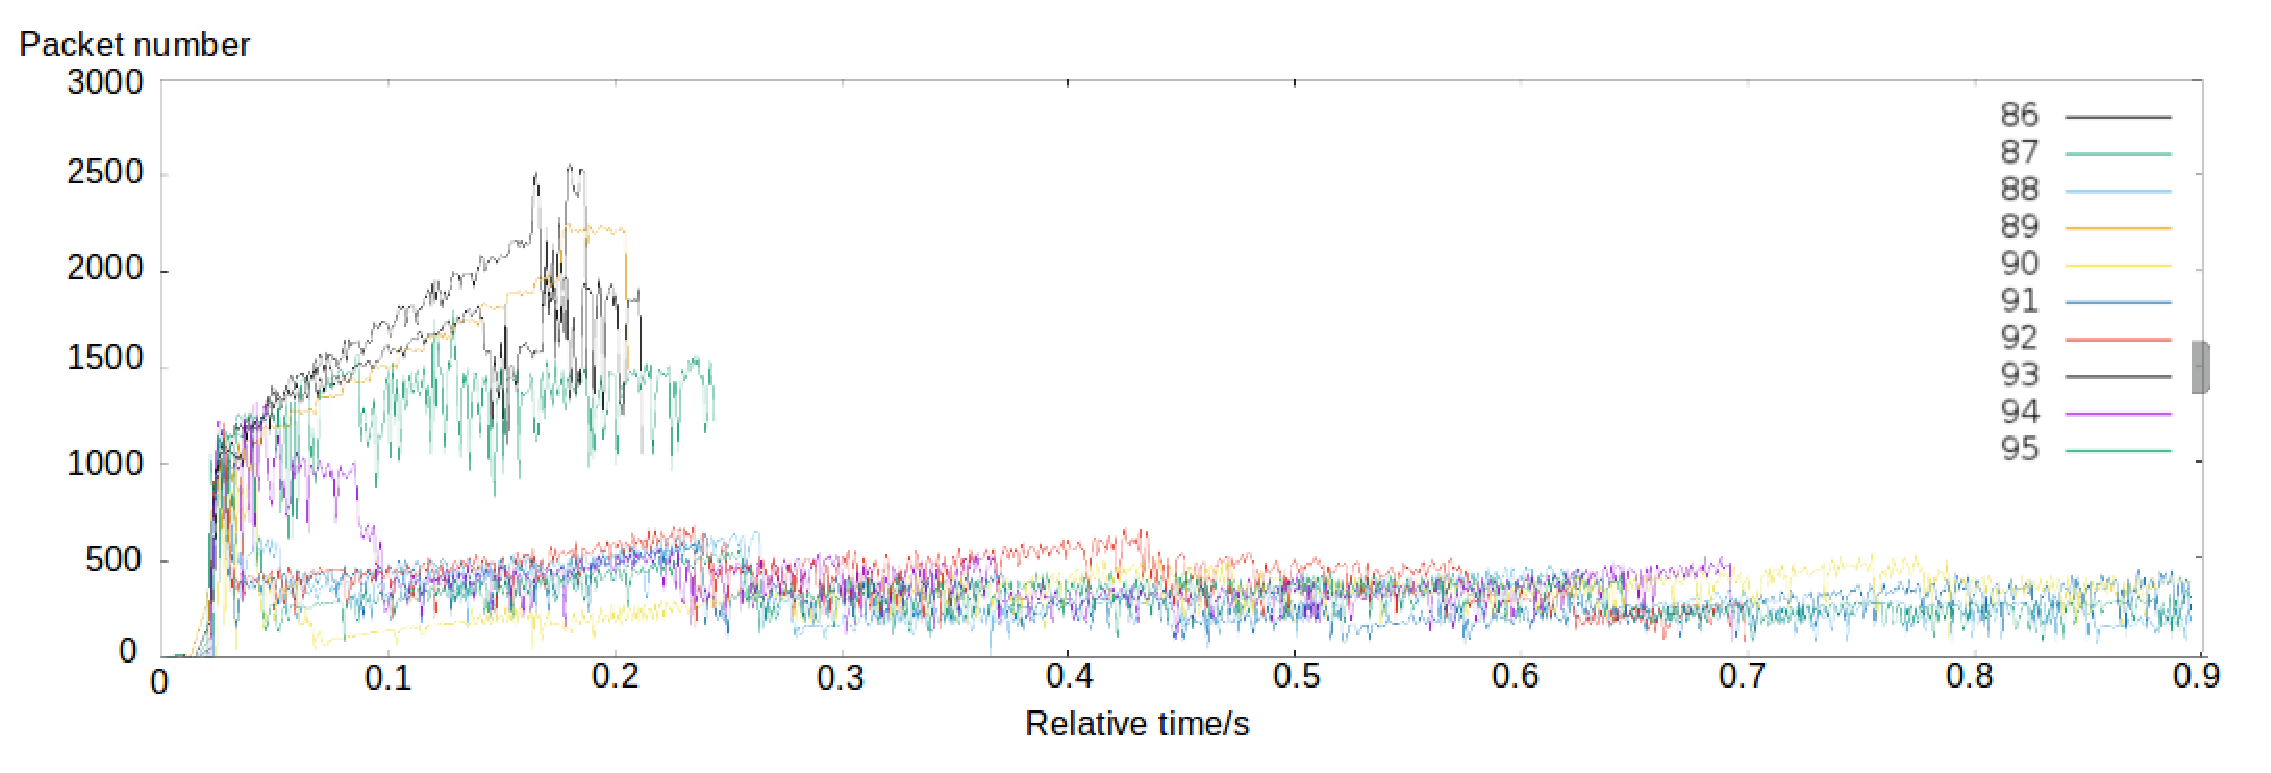
\includegraphics[width=6in]{10on1_1}
		\caption{10:1 incast bandwidth}
		\label{fig:10on1_1}
	\end{center}
\end{figure}

As we can see, the beginning parts are similar with 2:1 incast, but several flows fails to converge.
This is actually because of the Tcpdump covering range.
I set a limit for the number of packets captured by Tcpdump for each flow and that stops the figure of showing later bandwidth.

Later we try to draw bandwidth figures for more flows on the same machine.
We use 3 machines with each sending 20 flows at the same time and we get this in Figure ~\ref{fig:3_20_0}.

\begin{figure}[h!]
	\begin{center}
		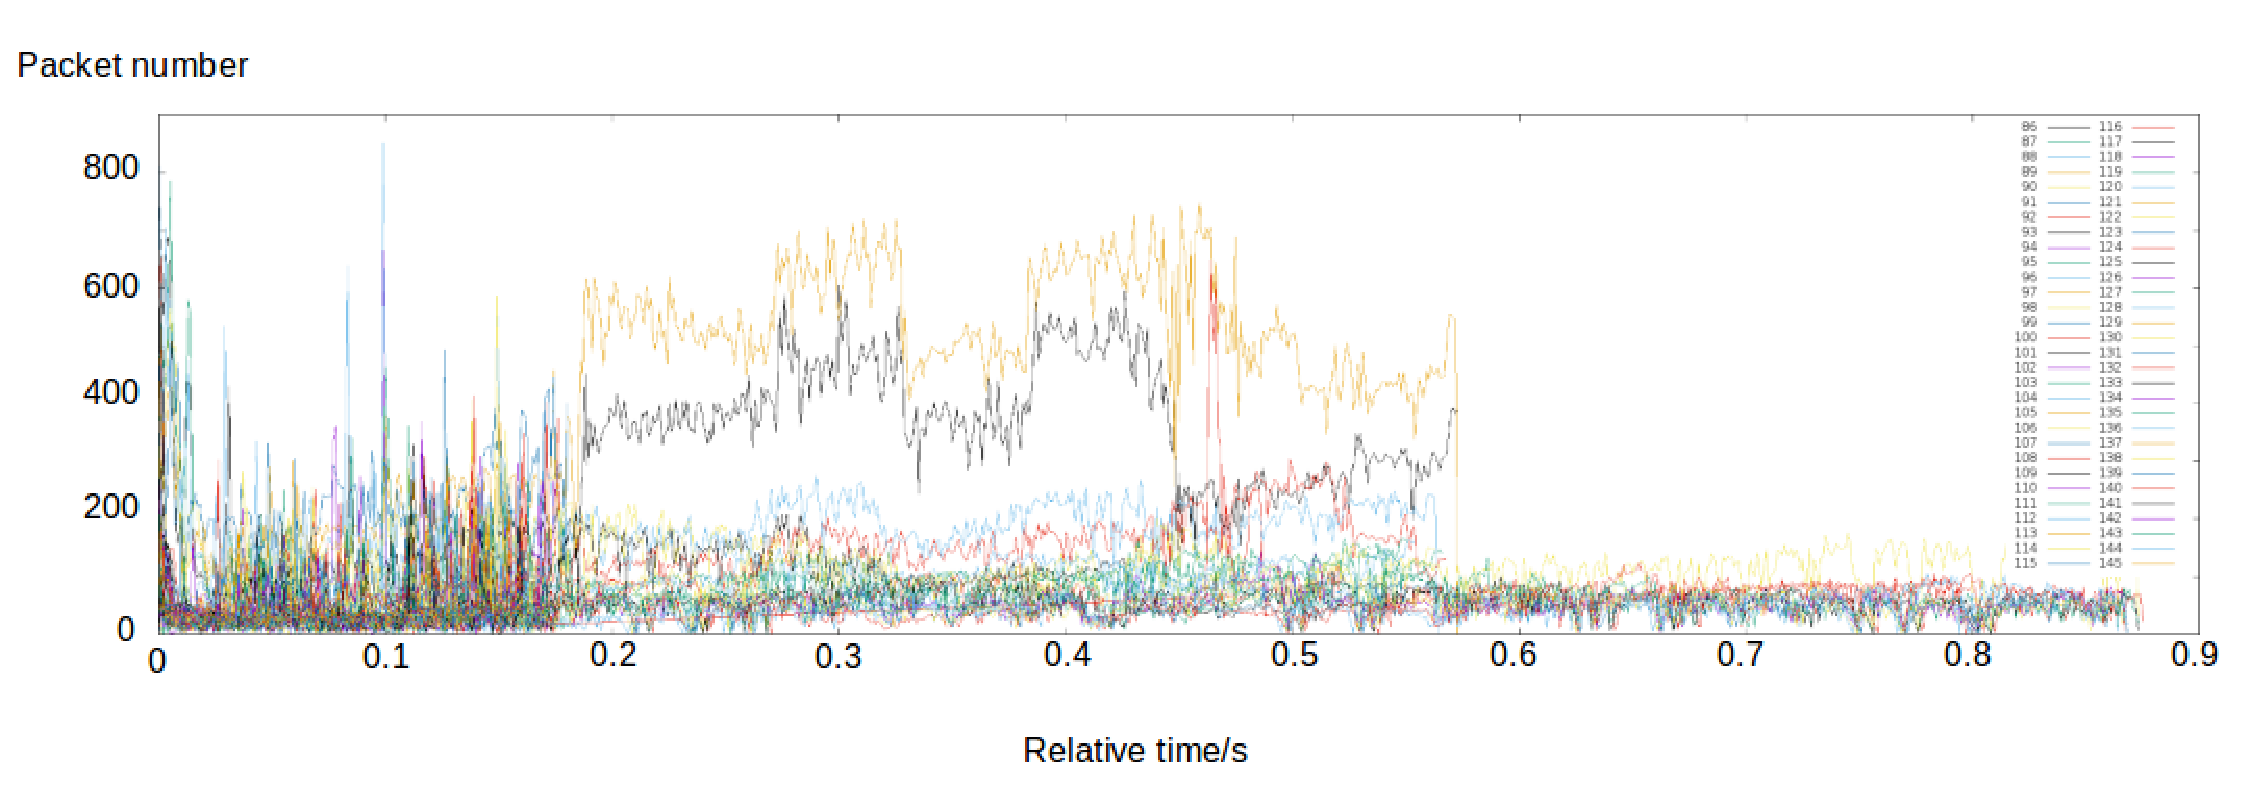
\includegraphics[width=6in]{3_20_0}
		\caption{60:1 incast bandwidth}
		\label{fig:3_20_0}
	\end{center}
\end{figure}

Although I have extended the capturing range a lot, the information can be grabbed from this figure is not much.
However, it's still obvious that the 60 flows converge within 0.5 seconds.
We should admit that the original DCQCN works for small-scale incast.

\subsection{Latency and Buffer Usage of Large-Scale Incast}
As the flow number grows larger, we find it hard to depict the bandwidth tendency using pictures.
There are mainly 2 reasons: too many lines override each other and we can't observe the tendency clearly, 
long capturing time makes the processing and figuring time extremely long (some may even last hours).

So we transfer to use latency and queue length to take a look at the large-scale incasts.
We are sending traffic for 80 seconds and pick 7 samples for each running starting from 10 seconds after flows start.
We execute 9 experiments, with each creating 80, 160, 240, ..., 720 flows.
That is, with 8 senders, each of the senders creates 10, 20, 30, ..., 90 flows.

With default paremeters coming from DCQCN, we get Table ~\ref{tab:default}.
From the table we can see the detailed buffer usage and latency conditions.
With the number of flows grows, the buffer and latency keep growing without control.

\begin{table}[h!]
	\begin{center}
		\caption{DCQCN buffer usage and latency}
		\label{tab:default}
		\begin{tabular}{|r|r|r|r|r|}
			\hline
			flow number & flow started & starting buffer & max buffer after 5s & average latency\\
			\hline
			$8\times 10$ & 80 & 457.5KB & 130.1KB & $24.84875\mu s$\\
			\hline
			$8\times 20$ & 160 & 4.9MB & 168.4KB & $31.784\mu s$\\
			\hline
			$8\times 30$ & 240 & 5.0MB & 195.4KB & $32.90625\mu s$\\
			\hline
			$8\times 40$ & 320 & 5.0MB & 267.4KB & $33.70875\mu s$\\
			\hline
			$8\times 50$ & 400 & 5.0MB & 388.9KB & $39.7225\mu s$\\
			\hline
			$8\times 60$ & 480 & 5.0MB & 591.4KB & $63.82875\mu s$\\
			\hline
			$8\times 70$ & 560 & 5.1MB & 858.0KB & $74.0024\mu s$\\
			\hline
			$8\times 80$ & 640 & 5.1MB & 1.2MB & $103.8075\mu s$\\
			\hline
			$8\times 90$ & 720 & 5.1MB & 5.1MB & $1792.83625\mu s$\\
			\hline
		\end{tabular}
	\end{center}
\end{table}

Those columns marked from 86 to 95 are average latency for flows on each machine.
86 to 95 are machine numbers.
I also use scripts to collect the number of flows that are successfully started to make sure that all flow start properly.

Then we apply some parameter changes to DCQCN+. To be more specific, they are listed as follows:
\begin{enumerate}
	\item DcQcnRateReduceMonitorPeriod, which the time period between rate reductions, is changed from $4\mu s$ to $40\mu s$.
	\item DcQcnTimeReset, which is the time period between rate increase events, is changed from $300\mu s$ to $3.1*flownum \mu s$.
	\item DcQcnAiRate, which is the rate increase step in Active Increase phase, is changed from $5Mbps$ to $\frac{256}{flownum} Mbps$.
\end{enumerate}
These are the only three parameters modifiable for our new algorithm and should contain more modifications if really applied to chips.

Thus we get Table ~\ref{tab:improved}.

\begin{table}[h!]
	\begin{center}
		\caption{DCQCN buffer usage and latency}
		\label{tab:improved}
		\begin{tabular}{|r|r|r|r|r|}
			\hline
			flow number & flow started & starting buffer & max buffer after 5s & average latency\\
			\hline
			$8\times 10$ & 80 & 1.0MB & 189.0KB & $27.2025\mu s$\\
			\hline
			$8\times 20$ & 160 & 4.7MB & 191.2KB & $31.0963\mu s$\\
			\hline
			$8\times 30$ & 240 & 4.8MB & 122.6KB & $29.9138\mu s$\\
			\hline
			$8\times 40$ & 320 & 4.7MB & 117.9KB & $29.9938\mu s$\\
			\hline
			$8\times 50$ & 400 & 4.9MB & 130.5KB & $30.1538\mu s$\\
			\hline
			$8\times 60$ & 480 & 4.9MB & 169.9KB & $30.4425\mu s$\\
			\hline
			$8\times 70$ & 560 & 5.0MB & 211.5KB & $31.9763\mu s$\\
			\hline
			$8\times 80$ & 640 & 5.0MB & 230.6KB & $31.74\mu s$\\
			\hline
			$8\times 90$ & 720 & 5.0MB & 681.8KB & $56.9813\mu s$\\
			\hline
		\end{tabular}
	\end{center}
\end{table}

We can see obvious difference between Figure ~\ref{tab:improved} and Figure ~\ref{tab:default}.
It's apparent that modified parameters provide shorter latency time and less buffer usage.
That marks the success of convergence and also demands reached for data center networks.

To take a closer look at the difference between the original DCQCN and DCQCN+.
We get the buffer usage difference in Figure ~\ref{fig:buffer} and latency difference in Figure ~\ref{fig:latency}.

\begin{figure}[h!]
	\begin{center}
		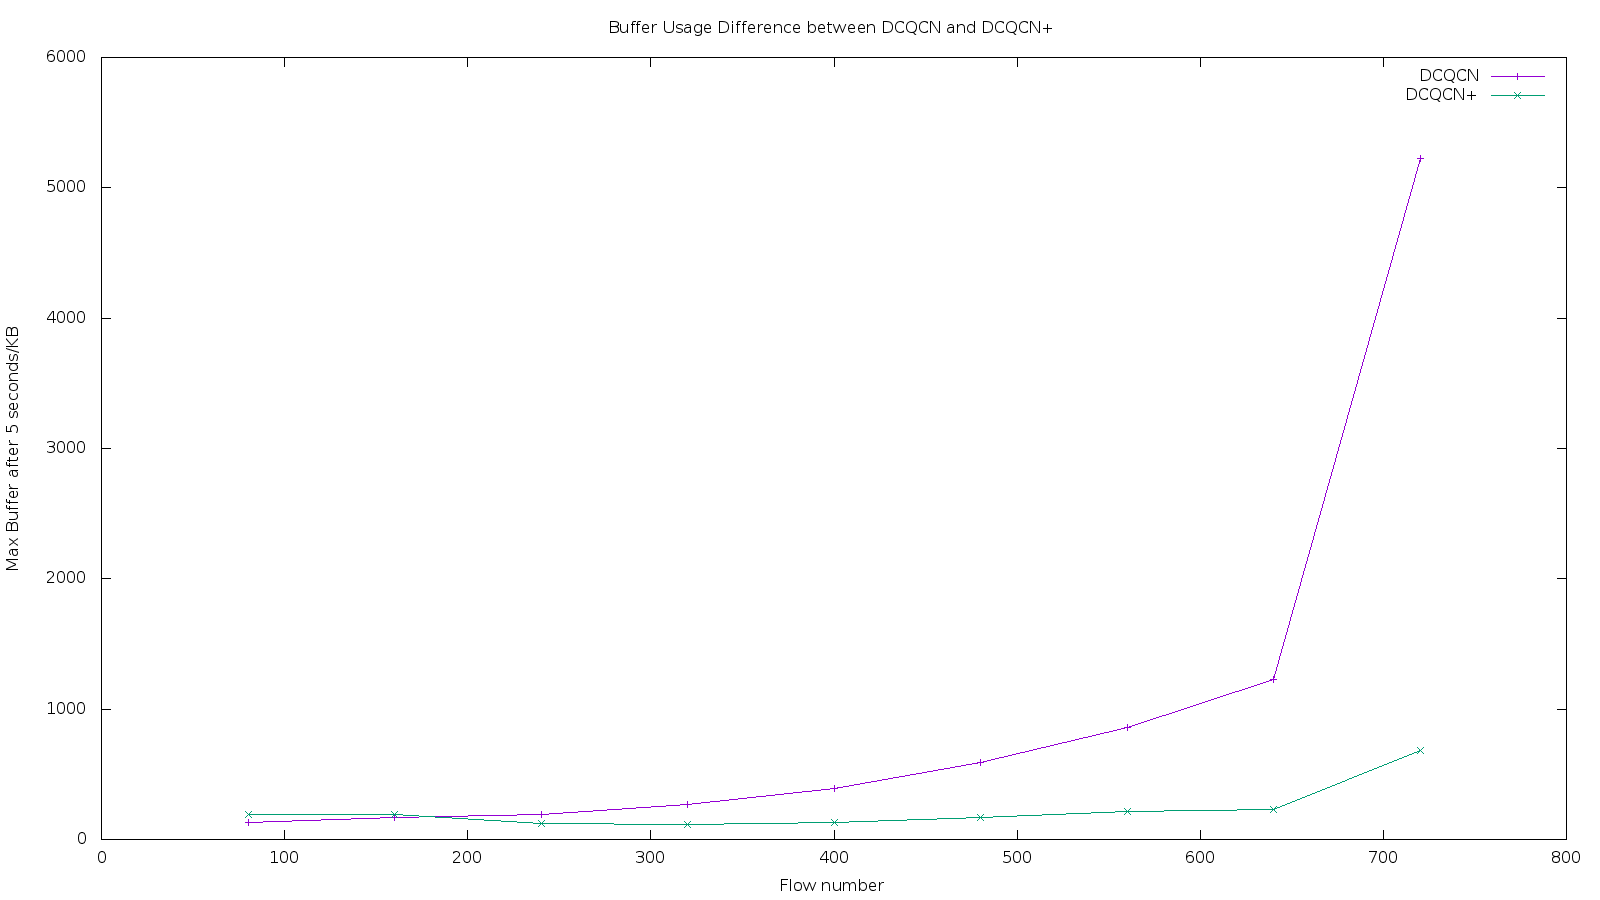
\includegraphics[width=6in]{buffer}
		\caption{Buffer usage difference between DCQCN and DCQCN+}
		\label{fig:buffer}
	\end{center}
\end{figure}

\begin{figure}[h!]
	\begin{center}
		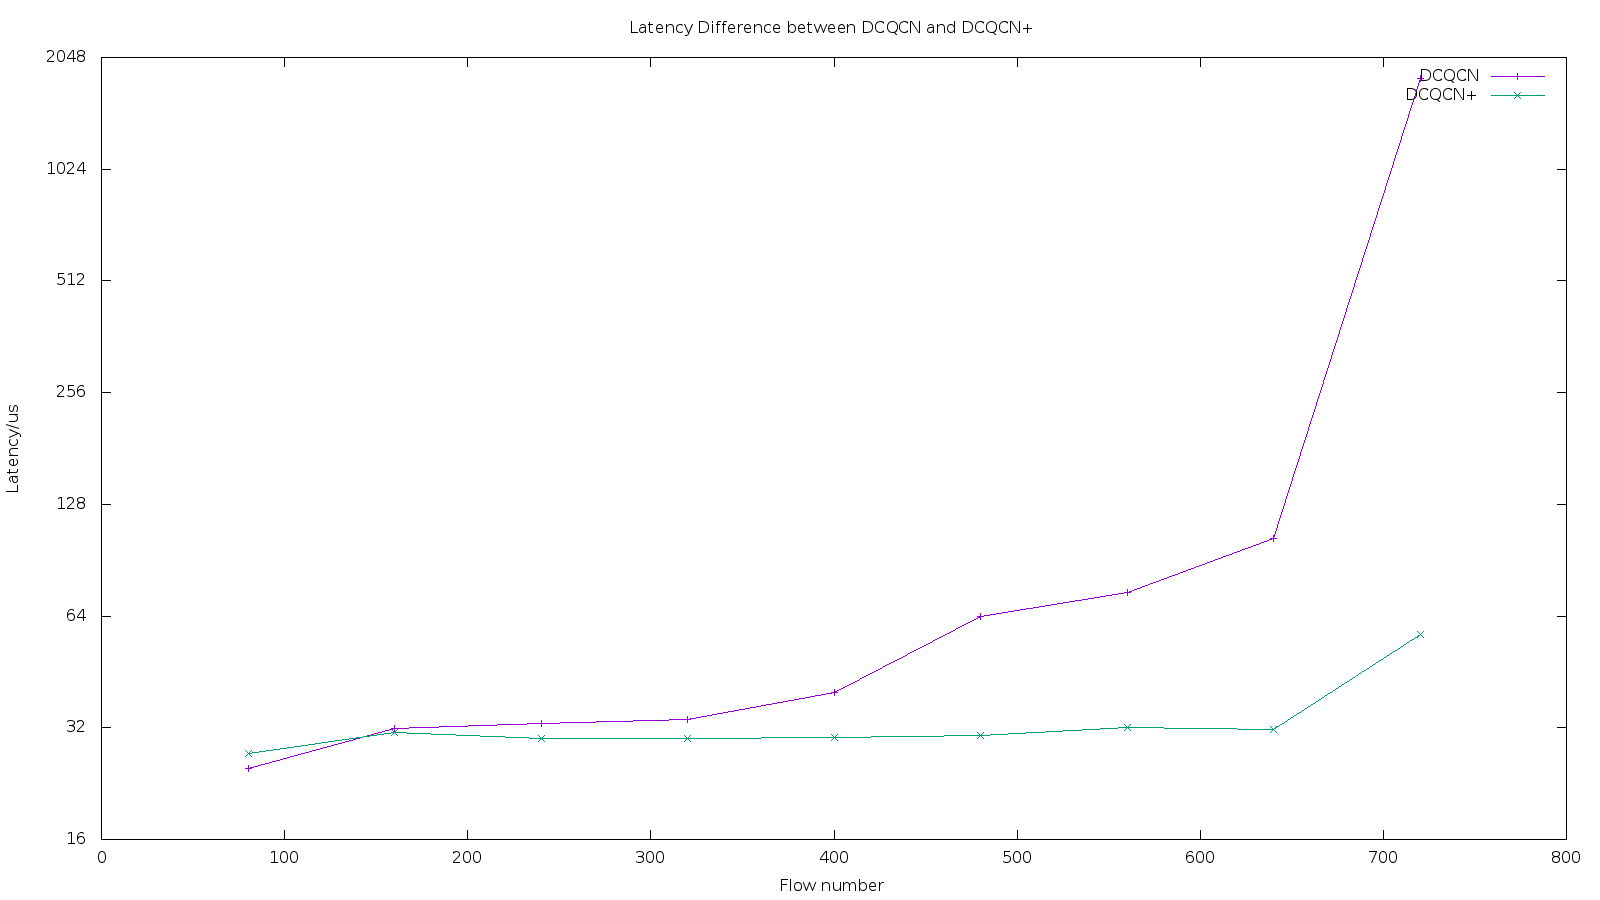
\includegraphics[width=6in]{latency}
		\caption{Latency difference between DCQCN and DCQCN+}
		\label{fig:latency}
	\end{center}
\end{figure}

To be clear, the buffer we collected is the maximal buffer usage 5 seconds after flows are started.
And in Figure ~\ref{fig:latency} the latency is depicted in exponential scaling to make the difference clearer.

We see that at the small scales, DCQCN+ seems to be worse than DCQCN.
That's actually the reason caused by parameter scaling.
The parameter scaling provided by Mellanox interface can't handle such accurate work, so I just pick the nearest integer,
which possibly cause the small disadvantage.

The buffer allocated by the switch is 5.1MB.
From Figure ~\ref{fig:buffer} we can know that the buffer usage reaches the maximum
and when the flow number reaches 720,
the convergence completely fails.
Actually for most cases, if the buffer usage maintains over 200KB, that's a failure of convergence.
Most large-scale incast is over the ability of DCQCN but can be controlled by DCQCN+.

\subsection{Results from NS3 Simulations}

Simulations are conducted by Dr. Yixiao Gao. The topology used is the same with Figure ~\ref{fig:Topology}.

With 8 senders starting a same number of flows at a uniform time within 0.1 seconds,
we can thus collect information easier than testbeds.
Four experiments are conducted with the flow number of 800, 1200, 1600 and 2000 respectively,
which means each of the senders starts 100, 150, 200, 250 flows respectively.

We get results with the link speed of 10Gbps and 40Gbps.

For link speed of 10Gbps, we get the queue length trends in Figure ~\ref{fig:simq10}
and throughput trends in Figure ~\ref{fig:simt10}.

For link speed of 10Gbps, we get the queue length trends in Figure ~\ref{fig:simq40}
and throughput trends in Figure ~\ref{fig:simt40}.

\begin{figure}[h!]
	\begin{center}
		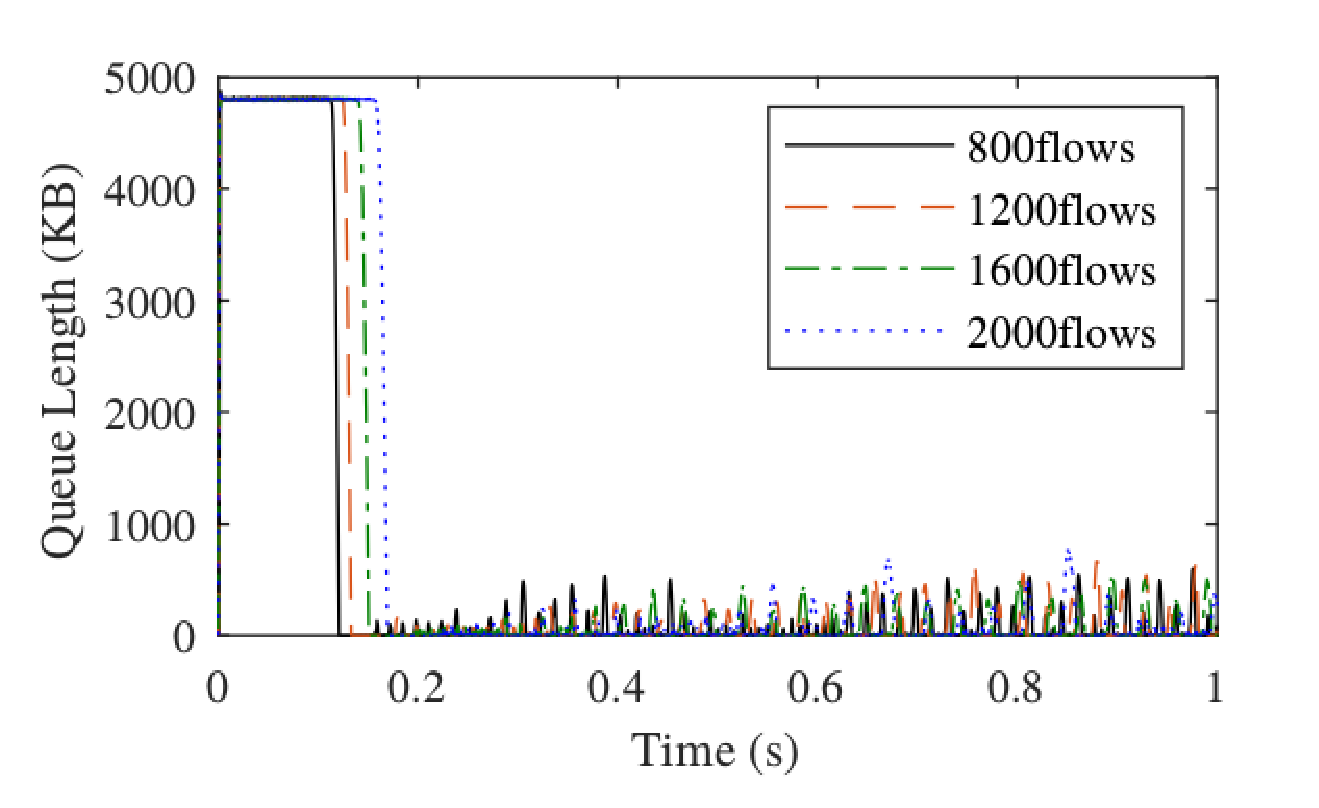
\includegraphics[width=6in]{simq10}
		\caption{Queue length trends of 10Gbps in DCQCN+}
		\label{fig:simq10}
	\end{center}
\end{figure}

\begin{figure}[h!]
	\begin{center}
		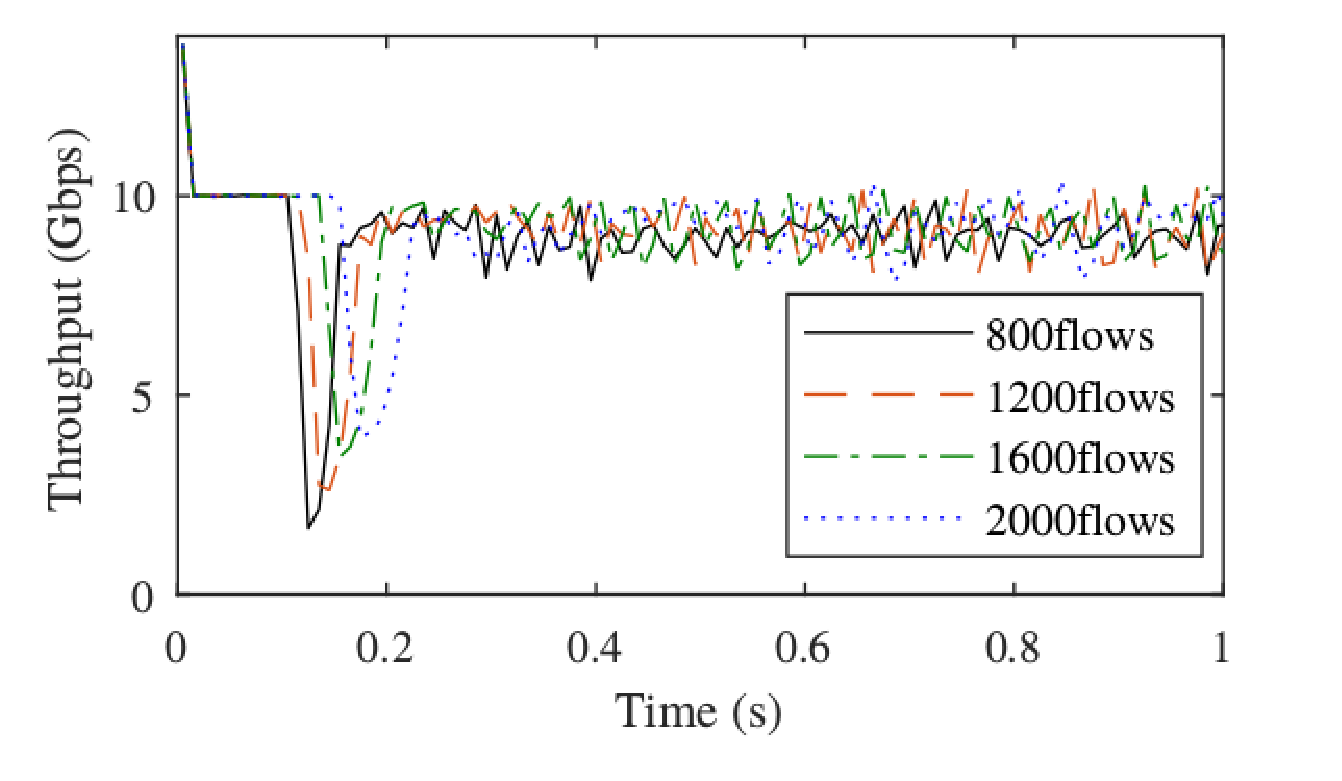
\includegraphics[width=6in]{simt10}
		\caption{Throughput trends of 10Gbps in DCQCN+}
		\label{fig:simt10}
	\end{center}
\end{figure}

\begin{figure}[h!]
	\begin{center}
		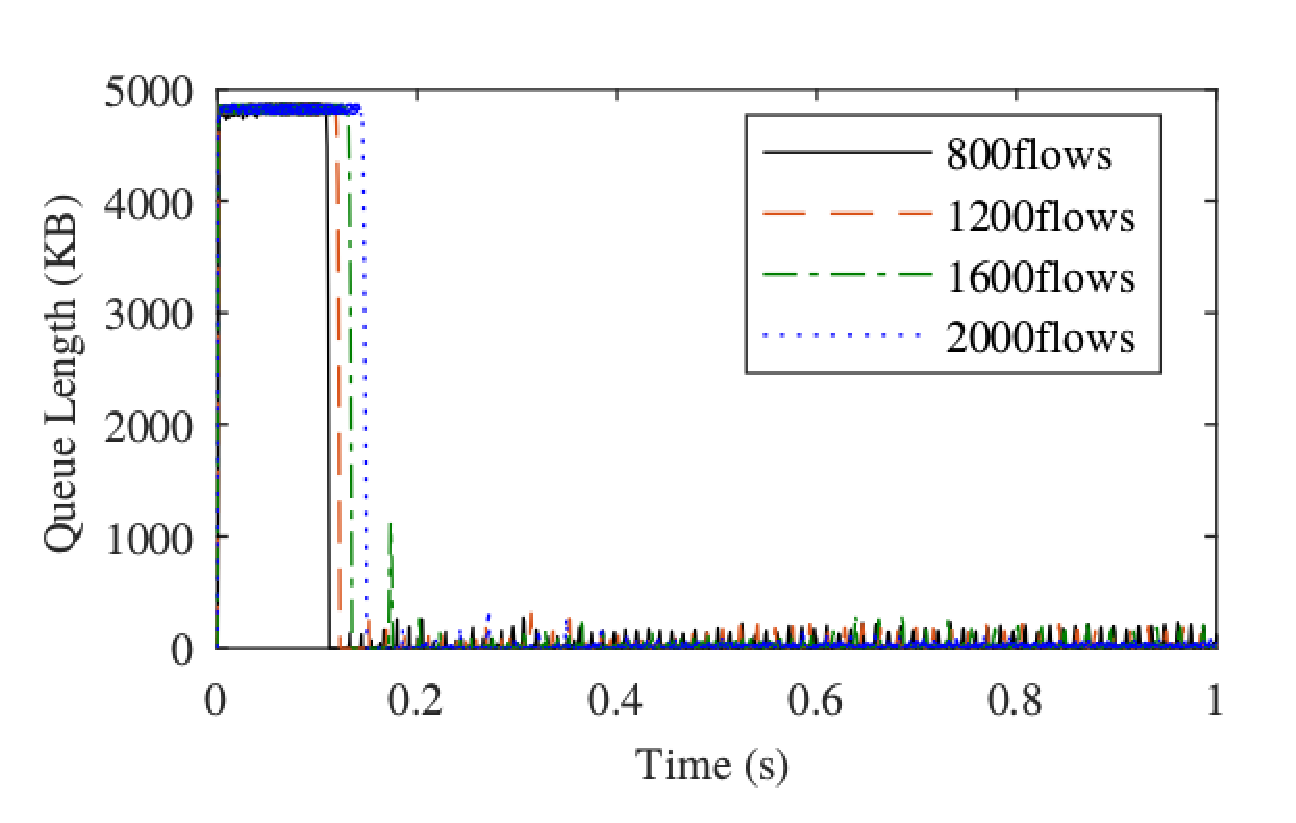
\includegraphics[width=6in]{simq40}
		\caption{Queue length trends of 40Gbps in DCQCN+}
		\label{fig:simq40}
	\end{center}
\end{figure}

\begin{figure}[h!]
	\begin{center}
		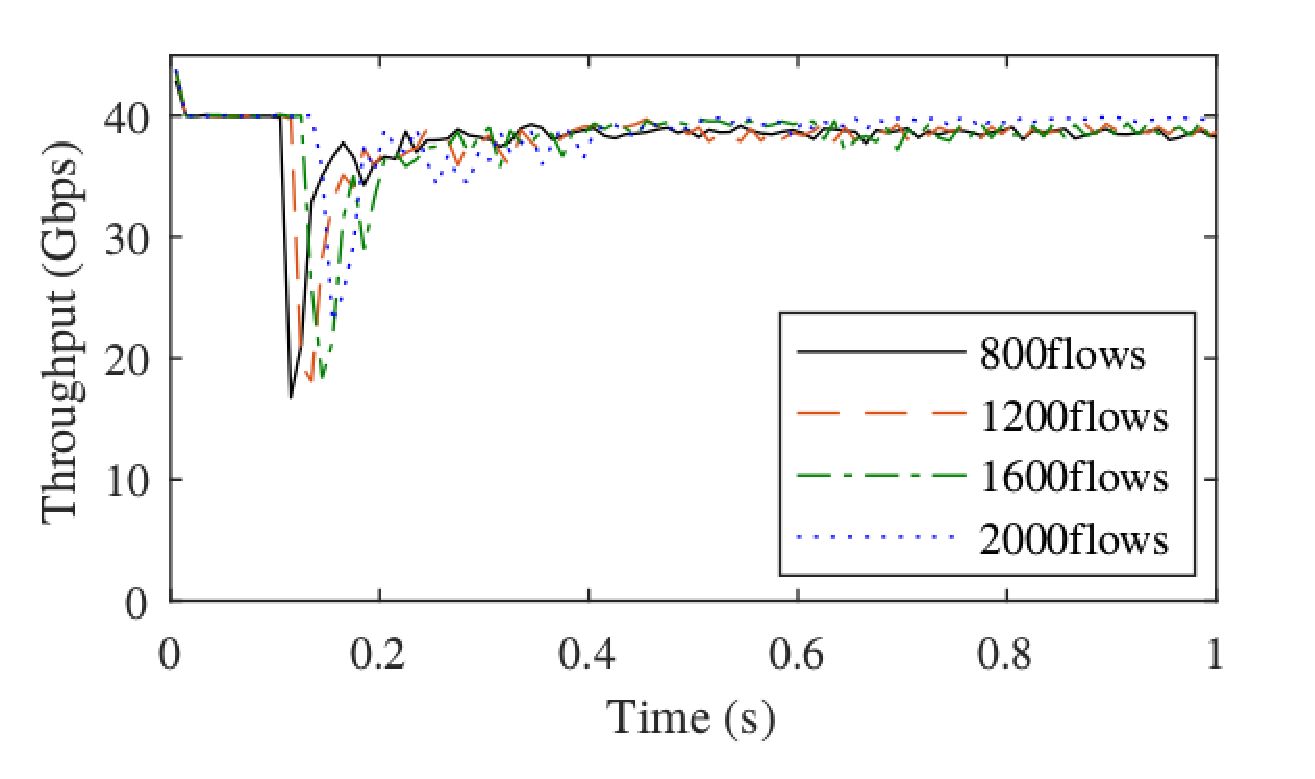
\includegraphics[width=6in]{simt40}
		\caption{Throughput trends of 40Gbps in DCQCN+}
		\label{fig:simt40}
	\end{center}
\end{figure}

We can see that the results are much better than the testbed results.
That makes sense since simulation does better in details.
Simulation can actually implement the timer updates mentioned in DCQCN+ but testbed can only use static parameters and some parameters
aren't accurate.

However, today's Data Center Network has hundreds or thougsands of hosts using CLOS \cite{CLOS} topology.
We also conduct experiments under the CLOS topology of 2410 nodes similar to CLOS \cite{CLOS}.
Average throughput when converged is about 95\%.

Compared with original DCQCN, DCQCN+ has 20 times smaller queue length, which is 20 times smaller queueing latency.


\newpage
\section{Conclusion and Future Work}

We have displayed the drawbacks of DCQCN.
When the network encounters large-scale traffic like an incast, DCQCN is forced to trigger PFC for a long time.
Such congestion control causes problems of high latency and buffer occupation.
We also conducted experiments to observe its features.
Then we develop DCQCN+, which does a better job in handling large-scale incasts and has similar performance with small incasts.
With adaptive parameter adjustments, DCQCN+ actually dynamically adjust congestion control scheme according to the incoming traffic.
We can see that DCQCN+ really does much better in latency and buffer usage.

Next steps of similar work should focus more on credit-based methods of congestion control schemes like \cite{credit}.
State-of-the-art methods do have better performance at the starting point.
However as the scale of traffic and data storage grows larger, bandwidth never becomes a problem.
People care more about latency and user experience.
The general case is that the growth of bandwidth is much faster than that of processing ability and buffer size.
What we are pursuing in the future is to explore in different schemes hoping to find a mixture of methods to relieve or even eliminate congestion.

\section*{Acknowledgement}

I greatly thank my advisor Prof. Chen Tian for his instructions and help all these years.
I also thank Dr. Yixiao Gao for instructing me on experiments and his great efforts on NS3 simulations.
Additionally, I need to thank Bo Li and other members in NASA group for their help in switch configurations and experiment executions.
I also appreciate Huawei Co. Ltd and Mellanox for their help during the process of the project.
Thanks for the support from my family, friends and other people who give me instructions and suggestions.


\bibliographystyle{IEEEtran}
\bibliography{report}


\end{document}
